\documentclass[a4paper,11pt]{article}

\usepackage[utf8]{inputenc}
\usepackage[T1]{fontenc}
\usepackage{lmodern}
\usepackage[margin=2.45cm]{geometry}
\usepackage{amsmath,amssymb,amsfonts,bm,mathtools}
\usepackage{amsthm}
\usepackage{graphicx}
\usepackage{booktabs}
\usepackage{array}
\usepackage{tabularx}
\usepackage{longtable}
\usepackage{siunitx}
\usepackage{xcolor}
\usepackage{hyperref}
\usepackage{enumitem}
\usepackage{physics}
\usepackage{placeins}
\usepackage{caption}
\usepackage{subcaption}

\numberwithin{equation}{section}
\sisetup{separate-uncertainty=true,per-mode=symbol,detect-all=true}
\hypersetup{colorlinks=true,linkcolor=blue,citecolor=blue,urlcolor=blue,
  pdftitle={Multilayer survival boundaries for quantum-enhanced Rayleigh-Doppler velocimetry},
  pdfauthor={Zhuoli Shu},
  pdfsubject={Quantum-enhanced Doppler velocimetry in photon-starved high-pressure gases}}

\newtheorem{proposition}{Proposition}

\newcommand{\Nret}{N_{\mathrm{ret}}}
\newcommand{\Nin}{N_{\mathrm{in}}}
\newcommand{\Ns}{N_{S}}
\newcommand{\Pzero}{P_{0}}
\newcommand{\etasys}{\eta_{\mathrm{sys}}}
\newcommand{\etas}{\eta_s}
\newcommand{\etai}{\eta_i}
\newcommand{\etaq}{\eta}
\newcommand{\Gammaeff}{\Gamma}
\newcommand{\GQ}{G_Q}
\newcommand{\Gtot}{G_Q^{\mathrm{tot}}}
\newcommand{\Geff}{G_{\mathrm{eff}}}
\newcommand{\FQ}{F_Q}
\newcommand{\FCS}{F_Q^{\mathrm{CS}}}
\newcommand{\FTMSV}{F_Q^{\mathrm{TMSV}}}
\newcommand{\Var}{\operatorname{Var}}
\newcommand{\RMSE}{\operatorname{RMSE}}
\newcommand{\Rguard}{R_{\mathrm{guard}}}
\newcommand{\Pwrap}{P_{\mathrm{wrap}}}
\newcommand{\SBR}{\mathrm{SBR}}
\newcommand{\repoURL}{\url{https://github.com/Pluviophiles-dev/Quantum_Doppler-Survival}}

\title{Multilayer survival boundaries for quantum-enhanced Rayleigh--Doppler velocimetry in photon-starved high-pressure gases}
\author{Zhuoli Shu\\
Independent Researcher\\
\texttt{shuzhuoli2@gmail.com}}
\date{May 31, 2026}

\begin{document}
\maketitle

\begin{abstract}
Clean high-pressure gas networks and hydrogen-blended pipelines need tracer-free velocity measurements, but molecular Rayleigh returns can fall into a photon-starved regime under restricted aperture, safe optical power, window loss, and finite detection efficiency. This paper studies whether a two-mode squeezed vacuum (TMSV) probe can retain a locally interpretable Rayleigh--Doppler phase-estimation advantage under these constraints. The analysis separates the macroscopic return-photon budget from the microscopic signal-mode resource, derives a closed-form one-sided-loss TMSV QFI advantage ratio, and keeps an equal-total-source-energy check for conservative accounting. Effective phase diffusion is treated as a first-order envelope tied to refractive-index wandering, while finite-dimensional QZZB checks, phase-wrapping tests, idler-loss scans, detector dark/background-count screens, and scenario tables are combined into a multilayer admissibility map. The result is not a single transmittance threshold: a surviving region must also pass diffusion, idler-preservation, detector, and global distinguishability checks. All numerical scripts, configuration files, data tables, and figure-generation routines are available in a public GitHub repository.
\end{abstract}

\section{Introduction: from a gas-measurement bottleneck to a multilayer survival problem}

High-pressure gas metrology, long-distance pipeline monitoring, and hydrogen-blended gas transport require velocity measurements that are non-invasive, stable, low-drift, and traceable. The practical pressure behind this problem is a traceability challenge: as transmission pressures rise and gas composition evolves, a future measurement chain must remain credible under high-pressure, clean, and potentially hydrogen-blended operating conditions. A tracer-free optical route would be attractive only if it respects the severe return-photon and detector constraints that such operating conditions impose.

Classical laser Doppler velocimetry (LDV) is mature when tracer particles provide strong Mie-scattering returns \cite{Durst1981,Albrecht2003,Tropea2007}. In clean high-pressure gas networks, however, filtration and cleanliness requirements can reduce the available particle population. Adding tracers is not always compatible with metrological traceability, gas quality, or operational constraints. Molecular Rayleigh scattering is therefore a natural non-invasive and tracer-free information carrier, but it is intrinsically weak compared with particle Mie scattering \cite{Miles2001,Gu2014,Witschas2011}. The problem then changes character: instead of asking how to process a strong particle-return LDV signal, one must ask whether a weak molecular-return optical phase can be estimated at all under realistic photon, loss, and detector constraints. Related optical gas diagnostics and primary-flow-metrology studies show that optical velocimetry in gases is physically meaningful, but the pressure, cleanliness, optical-access, and return-photon constraints are decisive \cite{Mickan2014,Maury2018}.

The photon budget is therefore not a peripheral engineering detail. Safe optical power, receiver aperture, window transmission, mode matching, detector efficiency, dark/background counts, and gate time can together determine whether the returned Rayleigh signal is statistically measurable. When the mean return photons per pulse are near or below unity, zero-count events and phase ambiguity enter the measurement problem. In this window, quantum enhancement is not a decorative upgrade to an already comfortable measurement. It is meaningful only as a boundary question: can nonclassical correlations remain useful after the weak-return optical, detector, loss, diffusion, and global-estimation layers have all been checked?

This paper asks the following boundary question. When Rayleigh return, detector noise, signal loss, idler loss, effective phase diffusion, and global phase ambiguity coexist, does there remain a reproducible, experimentally admissible, and locally interpretable quantum-advantage island? The question is deliberately narrower than instrument-level validation. It is also stricter than a pure quantum-channel calculation: the proposed boundary must survive not only loss-limited QFI, but also receiver-level admissibility and global distinguishability checks.

A boundary map is used rather than a direct performance claim for a specific instrument because the latter would require an end-to-end experimental platform, a detector POVM, field-qualified optical packaging, thermodynamic compensation, and full uncertainty budgeting. In the absence of such a platform, a direct prediction of industrial performance would be an overclaim. A falsifiable multilayer analysis is the appropriate intermediate object: it tells a future experiment when it is still meaningful to pursue a TMSV advantage, and when loss, diffusion, detector noise, idler degradation, or global ambiguity has already made that interpretation untenable.

The theoretical basis draws on several distinct lines of work. Quantum detection and estimation theory provide the statistical language for weak optical returns \cite{Helstrom1976,Holevo1982}. Noisy quantum metrology establishes that loss and decoherence can remove asymptotic Heisenberg-scaling advantages and impose channel-level precision limits \cite{Giovannetti2004,Giovannetti2011,Escher2011,Demkowicz2012,Demkowicz2015,Pezze2018}. Gaussian-state QFI and fidelity methods support the TMSV benchmark, covariance-matrix calculations, and composite-resource bookkeeping \cite{BraunsteinCaves1994,Paris2009,Monras2013,Safranek2019,Banchi2015,Weedbrook2012,Lu2012}. Phase-diffusion models motivate the treatment of refractive-index wandering as an effective dephasing process \cite{Genoni2011,Altorio2015,Pinel2013}. Bayesian and global bounds, especially Ziv--Zakai-type quantum bounds, identify regimes in which local QFI-based error propagation can become over-optimistic \cite{Tsang2012,Tsang2013}. Related weak-return quantum-sensing settings, such as quantum illumination and quantum target detection, further illustrate that a local advantage can be destroyed by loss, noise, and detection constraints \cite{Lloyd2008,Tan2008,Shapiro2020,Pirandola2018}.

The contributions are as follows:
\begin{enumerate}[label=(\roman*)]
  \item We propose a multilayer admissibility analysis that keeps Rayleigh photon budget, detector admissibility, TMSV QFI advantage, effective phase diffusion, idler preservation, phase wrapping, and QZZB checks rather than compressing them into a single loss parameter.
  \item We state a closed-form one-sided pure-loss TMSV survival threshold. Under equal signal-mode energy the SQL-equivalence boundary is $\etas=1/2$; under equal total source energy it approaches $\etas\simeq 0.75$ for large $\Ns$.
  \item We introduce a loss--diffusion survival island, $\Gamma < \ln \GQ(\etas,\Ns)$, and treat the phase-diffusion exponent as a sensitivity envelope rather than a universal constant.
  \item We use finite-dimensional diagnostic QZZB audits and phase-wrapping diagnostics to partition the local model into local-valid, guarded, and stop-extrapolation regions.
  \item We show that idler preservation is a second survival condition, not a secondary implementation detail.
  \item We provide scenario-level boundary tables and a public reproducibility package at \repoURL. The repository contains Python modules, configuration files, figure-generation scripts, tests, and processed numerical tables; the manuscript source files are not included in that public code repository.
\end{enumerate}

\begin{table}[htbp]
\centering
\caption{Claim ladder and evidence limits. The table separates manuscript-supported statements from conclusions that require additional instrumentation or experiments.}
\label{tab:claim_ladder}
\small
\renewcommand{\arraystretch}{1.12}
\begin{tabularx}{\textwidth}{p{0.27\textwidth}p{0.33\textwidth}X}
\toprule
Claim & Evidence in this work & What remains outside the claim \\
\midrule
Photon-starved Rayleigh windows can occur under constrained high-pressure gas optics & Rayleigh photon budget, zero-count probability, and worked 30 MPa anchors & Universal photon starvation for all industrial gas-metering configurations \\
A TMSV local QFI advantage can remain after one-sided loss & Closed-form pure-loss QFI ratio and equal-signal / equal-total resource thresholds & A detector-specific measurement attaining the QFI under all operating conditions \\
Effective phase diffusion imposes a finite survival island & Refractive-index-to-phase estimate, number-dephasing envelope, and exponent-sensitivity analysis & A full turbulence-resolved or non-Gaussian channel-QFI solution \\
Local RMSE propagation requires global checks & Phase-wrapping diagnostics and finite-dimensional diagnostic QZZB audits & A high-$N_S$ global optimality proof or certified attainable RMSE \\
Idler preservation is a second survival condition & Finite-dimensional idler-loss QFI map and covariance diagnostics & A complete receiver, storage, and mode-matching hardware design \\
Detector-level admissibility can veto otherwise favorable quantum-boundary points & Dark/background-count SBR screen and detector-margin map & A complete photon-counting POVM or field detector qualification \\
\bottomrule
\end{tabularx}
\end{table}

\begin{figure}[htbp]
  \centering
  
\includegraphics[width=0.95\textwidth]{figures/fig0_conceptual_schematic.png}
  \caption{System-level conceptual schematic of the boundary analysis. The signal mode probes the high-pressure gas and acquires Rayleigh--Doppler phase information under signal loss $\etas$ and effective phase diffusion $\Gamma$, while the idler mode is retained with efficiency $\etai$. The receiver layer is screened by detector-level dark/background-count admissibility. The decision layer separates the SQL benchmark, TMSV-QFI advantage, QZZB check, and stop-extrapolation regions. The diagram is a schematic of the modeling layers.}
  \label{fig:conceptual}
\end{figure}

\section{Photon-budget check and resource hierarchy}
\label{sec:budget}

The first layer is a macroscopic photon budget. It determines whether the proposed Rayleigh measurement is in a photon-rich, low-return, photon-starved, or extreme photon-starved window. This layer must not be confused with the microscopic signal-mode photon number used in the TMSV/coherent-state comparison.

\subsection{Rayleigh return photons and zero-count classification}

Let $\Nin$ be the number of emitted photons per probing pulse, $n(P,T)$ the molecular number density, $L$ the effective probe length, $\Omega$ the receiver solid angle, and $\etasys$ the aggregate macroscopic optical/detection efficiency. Under a single-scattering, homogeneous-medium approximation, the mean collected Rayleigh-return photons are
\begin{equation}
  \Nret = \Nin\, n(P,T)\, L\, \sigma_R(\lambda_0)\left(\frac{\Omega}{4\pi}\right)\etasys .
  \label{eq:rayleigh_budget}
\end{equation}
The single-molecule effective Rayleigh cross section is represented by
\begin{equation}
  \sigma_R(\lambda_0)=\frac{24\pi^3}{n_0^2\lambda_0^4}
  \left(\frac{n_{\mathrm{ref}}^2-1}{n_{\mathrm{ref}}^2+2}\right)^2 F_K,
  \label{eq:rayleigh_cross_section}
\end{equation}
which exposes the $\lambda_0^{-4}$ Rayleigh scaling. The number density in the numerical budget uses a Peng--Robinson methane proxy \cite{PengRobinson1976}. This proxy is a first-round density input for the photon-budget layer rather than a complete natural-gas thermodynamic model.

The zero-count probability is
\begin{equation}
  \Pzero=\exp(-\Nret).
\end{equation}
We use $\Pzero<1\%$ for photon-rich, $1\%\le\Pzero<37\%$ for low-return, $37\%\le\Pzero<90\%$ for photon-starved, and $\Pzero\ge90\%$ for extreme photon-starved. The classification is descriptive rather than universal; it is a reproducible way to connect mean return photons to empty-event risk.

\begin{table}[htbp]
\centering
\caption{Representative photon-budget inputs. The optimistic and constrained cases are separated to show that photon starvation is a boundary condition rather than an assumed universal state.}
\label{tab:photon_inputs}
\small
\begin{tabularx}{\textwidth}{l c l X}
\toprule
Parameter & Symbol & Value/range & Role \\
\midrule
Gas model & -- & pure methane proxy & first-round natural-gas density input \\
Pressure & $P$ & 1--35 MPa & controls molecular number density \\
Temperature & $T$ & 298.15 K & equation-of-state input \\
Wavelength & $\lambda_0$ & 532, 633, 1064, 1550 nm & Rayleigh scaling \\
Probe length & $L$ & 0.01 m & effective scattering length \\
Pulse energy & $E_p$ & $10^{-3}$ J / $10^{-6}$ J & optimistic / constrained cases \\
Collection fraction & $\Omega/4\pi$ & $10^{-6}$ / $10^{-7}$ & receiver geometry \\
System efficiency & $\etasys$ & 0.10 / 0.05 & macroscopic optical/detection efficiency \\
King factor & $F_K$ & 1.04 & methane anisotropy proxy \\
\bottomrule
\end{tabularx}
\end{table}

\begin{figure}[htbp]
  \centering
  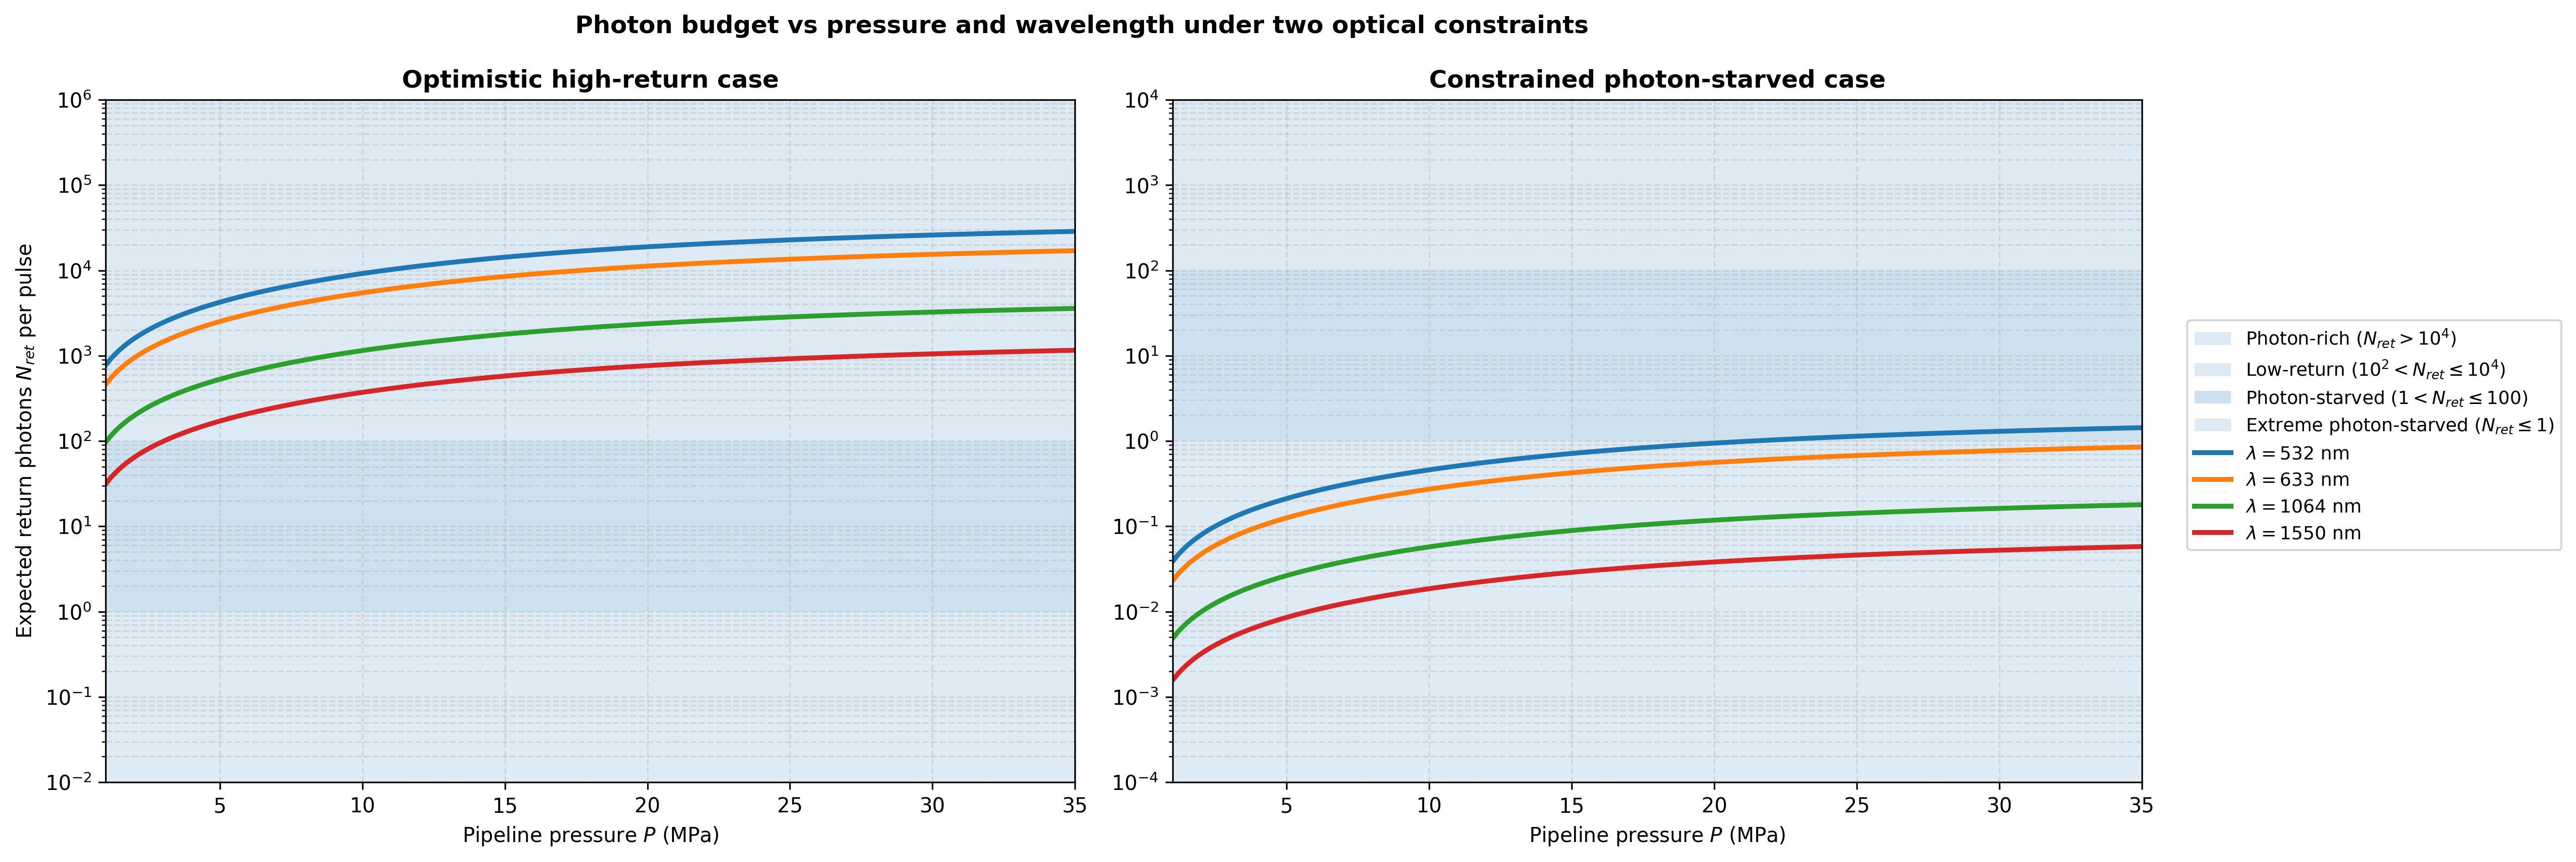
\includegraphics[width=0.95\textwidth]{fig1_photon_budget.png}
  \caption{Rayleigh return photon budget under two representative optical constraints. Panel A shows a favorable high-return optical case. Panel B shows a constrained photon-starved case. The horizontal bands indicate photon-rich, low-return, photon-starved, and extreme photon-starved regimes. The figure is a budget check, not a statement that all high-pressure gas velocimetry is photon-starved.}
  \label{fig:photon_budget}
\end{figure}

In the constrained case at $P=30~\mathrm{MPa}$, the reproduction script gives $\Nret\approx 1.30, 0.772, 0.163, 0.0526$ for $\lambda_0=532,633,1064,1550~\mathrm{nm}$, respectively. The corresponding zero-count probabilities are approximately $0.273,0.462,0.850,0.949$. This worked anchor is not meant to represent all industrial conditions. Its purpose is to provide a discrete, reproducible check that the photon-starved labels in Fig.~\ref{fig:photon_budget} follow from Eq.~\eqref{eq:rayleigh_budget} rather than from qualitative judgment.

\subsection{Photon-number and transmittance hierarchy}

The notation hierarchy is summarized in Table~\ref{tab:hierarchy}. The distinction is central to the paper. $\Nret$ is a macroscopic returned photon budget, while $\Ns$ is the signal-mode photon number in the microscopic quantum-estimation model. Likewise, $\etasys$ is a radiometric/detection efficiency in Eq.~\eqref{eq:rayleigh_budget}, while $\etas$ is a signal-mode quantum-channel transmittance in the QFI calculation.

This separation prevents two opposite mistakes. A reviewer should not use a small Rayleigh return, such as $\Nret\sim0.1$, to directly reject a microscopic comparison performed at $\Ns=100$, because the mapping from emitted probe state to collected Rayleigh return requires mode matching, temporal gating, scattering volume, receiver geometry, and detection statistics. Conversely, the author should not identify $\Nret$ with $\Ns$ and thereby imply an instrument model that has not been built. The present paper therefore keeps the two layers separate: $\Nret$ determines whether a gas-flow scenario is photon-starved and detector-admissible, while $\Ns$ determines the local quantum-estimation benchmark once a microscopic signal-mode resource has been specified.

\begin{table}[htbp]
\centering
\caption{Photon-number and transmittance hierarchy. These layers are intentionally not collapsed into a single effective parameter.}
\label{tab:hierarchy}
\small
\begin{tabularx}{\textwidth}{c X X X}
\toprule
Symbol & Layer & Role & What should not be done \\
\midrule
$\Nin$ & macroscopic emission & photon-budget input & do not treat it as the phase-estimation resource \\
$\Nret$ & macroscopic return & photon-starved classification & do not identify it with $\Ns$ \\
$\Ns$ & microscopic quantum probe & QFI/QZZB signal-mode resource & do not treat it as the Rayleigh return count \\
$\etasys$ & radiometric system efficiency & determines $\Nret$ & do not replace $\etas$ by $\etasys$ without a detector model \\
$\etas$ & signal-mode quantum channel & determines TMSV QFI survival & do not call it the total optical efficiency by default \\
$\etai$ & idler preservation & controls retained signal--idler correlation & do not assume it is automatically ideal \\
\bottomrule
\end{tabularx}
\end{table}

\subsection{Resource-accounting conventions}
\label{subsec:resource_accounting}

Two fairness conventions are used throughout the paper. The equal signal-mode energy criterion compares a coherent state and a TMSV probe with the same photon number entering the signal channel. This convention isolates whether the retained idler correlations improve phase estimation for a fixed signal-channel exposure. The equal total source energy criterion counts the TMSV idler photons as part of the resource cost and gives the coherent-state benchmark the corresponding total energy. This second criterion is more conservative and is retained as a resource-accounting check. Keeping both conventions prevents the survival boundary from depending on an unstated fairness assumption.

\section{Detector admissibility and coherent-state Doppler benchmark}
\label{sec:benchmark}

\subsection{Detector-level admissibility}

In a photon-starved window, detector dark counts and background counts can invalidate a budget point before any TMSV/QFI comparison is meaningful. We therefore treat them as a receiver-layer admissibility screen, not as an additional quantum-channel decoherence mechanism. For dark-count rate $R_{\mathrm{dark}}$, background rate $R_{\mathrm{bg}}$, and gate time $\tau_g$, define
\begin{equation}
  N_{\mathrm{noise}}=(R_{\mathrm{dark}}+R_{\mathrm{bg}})\tau_g,
  \qquad
  \SBR=\frac{\Nret}{N_{\mathrm{noise}}}.
  \label{eq:sbr}
\end{equation}
A point is detector-admissible only if $\SBR\ge \SBR_{\min}$ and $\Nret\ge N_{\mathrm{noise}}$. This condition does not modify the TMSV QFI formula; it asks whether the photon-budget layer remains experimentally measurable at the receiver.

\subsection{Doppler mapping and coherent-state SQL}

For scattering wave vector $\mathbf{q}=\mathbf{k}_s-\mathbf{k}_i$, the Doppler shift satisfies
\begin{equation}
  \Delta \omega_D=\mathbf{q}\cdot \mathbf{v},
  \qquad
  \phi=\Delta\omega_D\tau_{\mathrm{int}}.
\end{equation}
The estimated velocity component is the projection along $\mathbf{q}$,
\begin{equation}
  v_q=\frac{\phi}{|\mathbf{q}|\tau_{\mathrm{int}}},
  \qquad
  \sigma_{v_q}^2=\frac{\sigma_\phi^2}{|\mathbf{q}|^2\tau_{\mathrm{int}}^2}.
  \label{eq:phase_velocity}
\end{equation}
For the backscattering convention used in the numerical scripts,
\begin{equation}
  K_D=|\mathbf{q}|=\frac{4\pi n_g}{\lambda_0}.
\end{equation}
The coherent-state SQL benchmark under signal transmittance $\etas$ and $M$ independent samples is
\begin{equation}
  \FCS=4\etas\Ns,
  \qquad
  \Var(\hat\phi)_{\mathrm{CS}}\ge \frac{1}{4M\etas\Ns}.
  \label{eq:coherent_sql}
\end{equation}
This benchmark is the normalization reference for the TMSV advantage ratios below. The SQL propagation plot is retained in Appendix~\ref{app:detector_macro} because it is a baseline rather than a main survival result.

\begin{table}[htbp]
\centering
\caption{Baseline comparison and failure modes. The proposed TMSV route is positioned relative to classical particle LDV, coherent Rayleigh probing, detector-limited measurements, and local-QFI-only predictions.}
\label{tab:baseline_comparison}
\scriptsize
\begin{tabularx}{\textwidth}{p{0.19\textwidth}p{0.20\textwidth}p{0.20\textwidth}p{0.22\textwidth}X}
\toprule
Approach & Information carrier & Strength & Failure mode & Role here \\
\midrule
Particle/Mie LDV & tracer particles & mature and strong return & requires particles/tracers & external classical reference \\
Coherent Rayleigh probe & molecular Rayleigh return & tracer-free SQL baseline & photon-starved under constrained optics & normalization benchmark \\
TMSV Rayleigh probe & signal--idler correlations & possible local QFI gain & loss, diffusion, idler degradation & candidate quantum probe \\
TMSV with poor idler preservation & degraded correlations & reduced or no advantage & $\eta_i$ too low & rejected by idler screen \\
Detector-limited Rayleigh measurement & weak photon return plus counts & physically motivated low-return case & dark/background counts dominate & vetoed before QFI interpretation \\
Local-QFI-only prediction & derivative-based local bound & analytic and simple & phase wrapping/global ambiguity & guarded by QZZB check \\
\bottomrule
\end{tabularx}
\end{table}

\section{Proposition 1: one-sided-loss TMSV survival threshold}
\label{sec:tmsv_qfi}

A zero-mean TMSV state with signal-mode photon number $\Ns$ has covariance matrix, in the $\hbar=2$ convention,
\begin{equation}
V_0=
\begin{pmatrix}
(2\Ns+1)I_2 & 2\sqrt{\Ns(\Ns+1)}Z_2\\
2\sqrt{\Ns(\Ns+1)}Z_2 & (2\Ns+1)I_2
\end{pmatrix},
\quad Z_2=\mathrm{diag}(1,-1).
\end{equation}
Under one-sided signal loss with transmittance $\etas$, the output covariance matrix is
\begin{equation}
V_{\eta}=
\begin{pmatrix}
[1+2\etas\Ns]I_2 & 2\sqrt{\etas\Ns(\Ns+1)}Z_2\\
2\sqrt{\etas\Ns(\Ns+1)}Z_2 & (2\Ns+1)I_2
\end{pmatrix}.
\end{equation}

\begin{proposition}[Equal-signal-energy survival threshold under one-sided pure loss]
Consider local phase estimation in which the unknown phase is encoded only on the signal mode of a TMSV probe. The signal mode undergoes a one-sided vacuum pure-loss channel with transmittance $\etas$, the idler is ideally preserved, and the comparison coherent state uses the same signal-mode photon number $\Ns$. Then the TMSV QFI is
\begin{equation}
  F_Q^{\mathrm{TMSV,loss}}=\frac{4\etas\Ns(\Ns+1)}{1+2(1-\etas)\Ns},
  \label{eq:tmsv_qfi}
\end{equation}
while the coherent-state benchmark is $F_Q^{\mathrm{CS}}=4\etas\Ns$. The corresponding equal-signal-energy advantage ratio is
\begin{equation}
  \GQ(\etas,\Ns)=\frac{F_Q^{\mathrm{TMSV,loss}}}{F_Q^{\mathrm{CS}}}
  =\frac{\Ns+1}{1+2(1-\etas)\Ns}.
  \label{eq:gq}
\end{equation}
The SQL-equivalence boundary under this criterion is $\etas=1/2$. Under equal total source energy, the advantage ratio becomes
\begin{equation}
  \Gtot(\etas,\Ns)=\frac{\Ns+1}{2[1+2(1-\etas)\Ns]},
  \qquad
  \eta_c^{\mathrm{tot}}=\frac{3}{4}+\frac{1}{4\Ns}.
  \label{eq:gtotal}
\end{equation}
For large $\Ns$, the conservative equal-total-energy threshold approaches $\etas\simeq0.75$.
\end{proposition}

The loss channel reduces more than the mean signal energy. The vacuum mode injected by one-sided loss also dilutes the signal--idler covariance terms that carry the phase-sensitive EPR correlations, lowers the output purity, and suppresses the QFI gain. The boundary $\etas=1/2$ should therefore be read as a channel-level survival threshold under the equal-signal-energy convention, not as a numerical fitting artifact. The equal-total-source-energy check is included because a TMSV source consumes an idler mode in addition to the signal mode.

\begin{figure}[htbp]
  \centering
  
\includegraphics[width=0.95\textwidth]{fig3_pure_loss_tmsv.png}
  \caption{Pure-loss TMSV advantage window. The left panel zooms into the transition near $\GQ=1$ for representative $\Ns$, while the inset preserves the high-transmittance tail. The right panel shows the topology of $\GQ(\etas,\Ns)$, with colors clipped to emphasize the boundary near $\etas=0.5$. The conservative equal-total-source-energy threshold is also indicated.}
  \label{fig:pure_loss}
\end{figure}

\section{Effective phase diffusion as a boundary surrogate}
\label{sec:diffusion}

\subsection{Physical bridge from refractive-index wandering to phase diffusion}

Refractive-index wandering in high-pressure gas produces random optical path fluctuations. If $\delta n(z,t)$ is the refractive-index fluctuation along an effective path length $L$, then
\begin{equation}
  \delta\phi(t)=k_0\int_0^L\delta n(z,t)\,dz,
  \qquad k_0=\frac{2\pi}{\lambda_0}.
\end{equation}
Under weak-scattering, short-integration, and coarse-grained conditions, the accumulated random phase variance can be summarized by an effective phase-diffusion strength
\begin{equation}
  \Gamma=\gamma_\phi\tau_{\mathrm{int}}.
\end{equation}
A number-operator dephasing channel can be written in GKLS form as
\begin{equation}
  \frac{d\rho}{dt}=-i[\hat n,\rho]+\mathcal{D}[\sqrt{\gamma_\phi}\hat n]\rho.
\end{equation}
In the number basis this suppresses off-diagonal elements as
\begin{equation}
  \rho_{n,m}(t)=\exp\!\left[-\frac{\Gamma}{2}(n-m)^2\right]\rho_{n,m}(0).
  \label{eq:number_dephasing}
\end{equation}

\paragraph{Auditable order-of-magnitude link to gas refractivity.}
The dimensionless diffusion coordinate $\Gamma$ is abstract only if it is left disconnected from gas physics. A minimal refractivity estimate can be obtained from the phase variance induced by a random refractive-index field. Let
\begin{equation}
  C_n(\Delta z)=\langle \delta n(z)\delta n(z+\Delta z)\rangle
\end{equation}
be the longitudinal refractive-index covariance over the effective optical path. Then
\begin{equation}
  \mathrm{Var}(\delta\phi)=k_0^2\int_0^L\!\int_0^L C_n(z-z')\,dz\,dz'.
  \label{eq:phase_variance_index}
\end{equation}
For a correlation length $L_c\ll L$ and rms refractivity fluctuation $\sigma_n$, an exponential or compactly supported covariance gives the reproducible scaling
\begin{equation}
  \Gamma_n \sim C_c k_0^2 L L_c \sigma_n^2,
  \qquad C_c=\mathcal{O}(1),
  \label{eq:gamma_refractivity_scaling}
\end{equation}
where the order-unity coefficient depends on the chosen covariance shape and on how phase variance is mapped to the number-dephasing coordinate. This estimate is not a turbulence model. It is a bridge that lets the survival island be read against gas parameters: pressure, temperature, composition, and turbulent mixing enter through $\sigma_n$ and $L_c$. In a Lorentz--Lorenz linearization one may write schematically
\begin{equation}
  \sigma_n^2 \simeq
  \left(\frac{\partial n}{\partial \rho}\right)^2\sigma_\rho^2+
  \left(\frac{\partial n}{\partial T}\right)^2\sigma_T^2+
  \left(\frac{\partial n}{\partial x_{\mathrm{H}_2}}\right)^2\sigma_x^2+\cdots,
\end{equation}
so higher pressure and hydrogen-blending variability can increase the need for an explicit diffusion check. For $\lambda_0=1064\,\mathrm{nm}$, $L=1\,\mathrm{cm}$, and $L_c=1\,\mathrm{mm}$, Eq.~\eqref{eq:gamma_refractivity_scaling} gives approximately $\Gamma_n\sim3.5\times10^{-4},3.5\times10^{-2},3.5$ for $\sigma_n=10^{-6},10^{-5},10^{-4}$, respectively. Thus the plotted $\Gamma$ axis spans weak refractivity wandering through a regime where diffusion can erase the local TMSV advantage.

\paragraph{Why an exponential envelope?}
The exponential factor in $\Geff=\GQ e^{-\Gamma}$ is not introduced as an exact non-Gaussian channel-QFI solution. It is used as a first-order boundary envelope. Equation~\eqref{eq:number_dephasing} shows that accumulated number dephasing progressively suppresses number-basis coherences. The pure-loss TMSV advantage is carried by phase-sensitive signal--idler correlations; once these coherences are reduced, the advantage ratio should depend on more than the loss parameter $\eta_s$. The envelope projects this leading coherence-suppression intuition onto the advantage ratio. It is therefore a survival-screening condition rather than a precision prediction.

The finite-dimensional exact dephasing-QFI sanity checks in Appendix~\ref{app:diffusion} confirm the intended role of the envelope: the exact truncated-Fock QFI decreases monotonically with $\Gamma$ and does not revive advantage when the pure-loss ratio is already at or below the SQL boundary. The numerical values are not required to match the envelope coefficient; the envelope is used to classify survival topology, not to fit the exact non-Gaussian QFI.

\subsection{Loss--diffusion survival island}

The baseline local survival envelope is
\begin{equation}
  \Geff(\etas,\Ns,\Gamma)=\GQ(\etas,\Ns)e^{-\Gamma}.
  \label{eq:geff}
\end{equation}
Solving $\Geff=1$ gives
\begin{equation}
  \Gamma_{\max}(\etas,\Ns)=\ln \GQ(\etas,\Ns),\qquad \GQ>1.
  \label{eq:gamma_max}
\end{equation}
If $\GQ\le1$, no phase-diffusion convention can recover a TMSV advantage in this first-order boundary model. To expose the sensitivity to the exponent convention, Appendix~\ref{app:diffusion} uses
\begin{equation}
  \Geff^{(a)}=\GQ e^{-a\Gamma},\qquad a\in\{1/2,1,2\}.
\end{equation}
For $\Ns=100$ and $\etas=0.90$, $\GQ=4.8095$ and the baseline $a=1$ boundary is $\Gamma_{\max}=1.5706$. The sensitivity envelope gives $\Gamma^{(1/2)}_{\max}=3.1412$, $\Gamma^{(1)}_{\max}=1.5706$, and $\Gamma^{(2)}_{\max}=0.7853$. Thus the exponent coefficient changes the width of the island but not the existence of a finite loss--diffusion boundary.

A local Gaussian phase estimator becomes unsafe when the phase error is comparable to the interferometric period. We therefore monitor
\begin{equation}
  \Pwrap=\Pr(|\Delta\phi|>\pi)=\operatorname{erfc}\left(\frac{\pi}{\sqrt{2}\sigma_\phi}\right).
\end{equation}
The loss-diffusion plot must be read together with phase-wrapping contours and QZZB checks.

\begin{figure}[htbp]
  \centering
  
\includegraphics[width=0.95\textwidth]{fig4_survival_wrapping_bridge.png}
  \caption{Loss--diffusion survival island and phase-wrapping bridge. Panel (a) shows the first-order effective advantage $\Geff$ for $\Ns=100$. Panel (b) shows analytic survival-boundary curves. Panel (c) overlays phase-wrapping risk and representative finite-dimensional diagnostic QZZB guard-check points. The figure connects local survival to global checks; it is not a full non-Gaussian QZZB solution.}
  \label{fig:survival_wrapping}
\end{figure}

\section{Multilayer admissibility map and scenario-level verdicts}
\label{sec:multilayer}

The preceding layers can be combined into an admissible-region definition. Let $\mathcal{S}_{\mathrm{adm}}$ be the set of parameter points satisfying
\begin{align}
  \Nret &\in \text{an reproducible low-return or photon-starved budget window},\nonumber\\
  \SBR=\Nret/N_{\mathrm{noise}} &\ge \SBR_{\min},\nonumber\\
  \Geff(\etas,\Ns,\Gamma)&>1,\nonumber\\
  \Pwrap&<P_{\mathrm{th}},\nonumber\\
  \Rguard&<R_{\mathrm{th}},\nonumber\\
  \etai&\ge \eta_{i,\min}.
  \label{eq:admissible_set}
\end{align}
This definition is not a theorem of optimal detection. It is a transparent survival check. Each layer vetoes a different failure mode: detector-limited return, idler degradation, no local QFI advantage, phase/wrapping stop, guarded boundary, or locally interpretable region.

\paragraph{Algorithm 1: multilayer survival classification.}
The numerical classification follows a transparent sequence: (1) compute $\Nret$ and $P_0$ from the Rayleigh budget; (2) check detector admissibility using Eq.~\eqref{eq:sbr}; (3) evaluate the pure-loss ratio $\GQ$ and reject points with no local channel advantage; (4) apply the diffusion envelope $\Geff>1$; (5) check idler preservation; (6) evaluate phase-wrapping risk; (7) apply the QZZB guard ratio where available; and (8) assign the verdict local-valid, guarded, detector-limited, idler-limited, or stop-extrapolation. This algorithmic view is important: the multilayer map is not a single formula, but a reproducible decision procedure.

\begin{figure}[htbp]
  \centering
  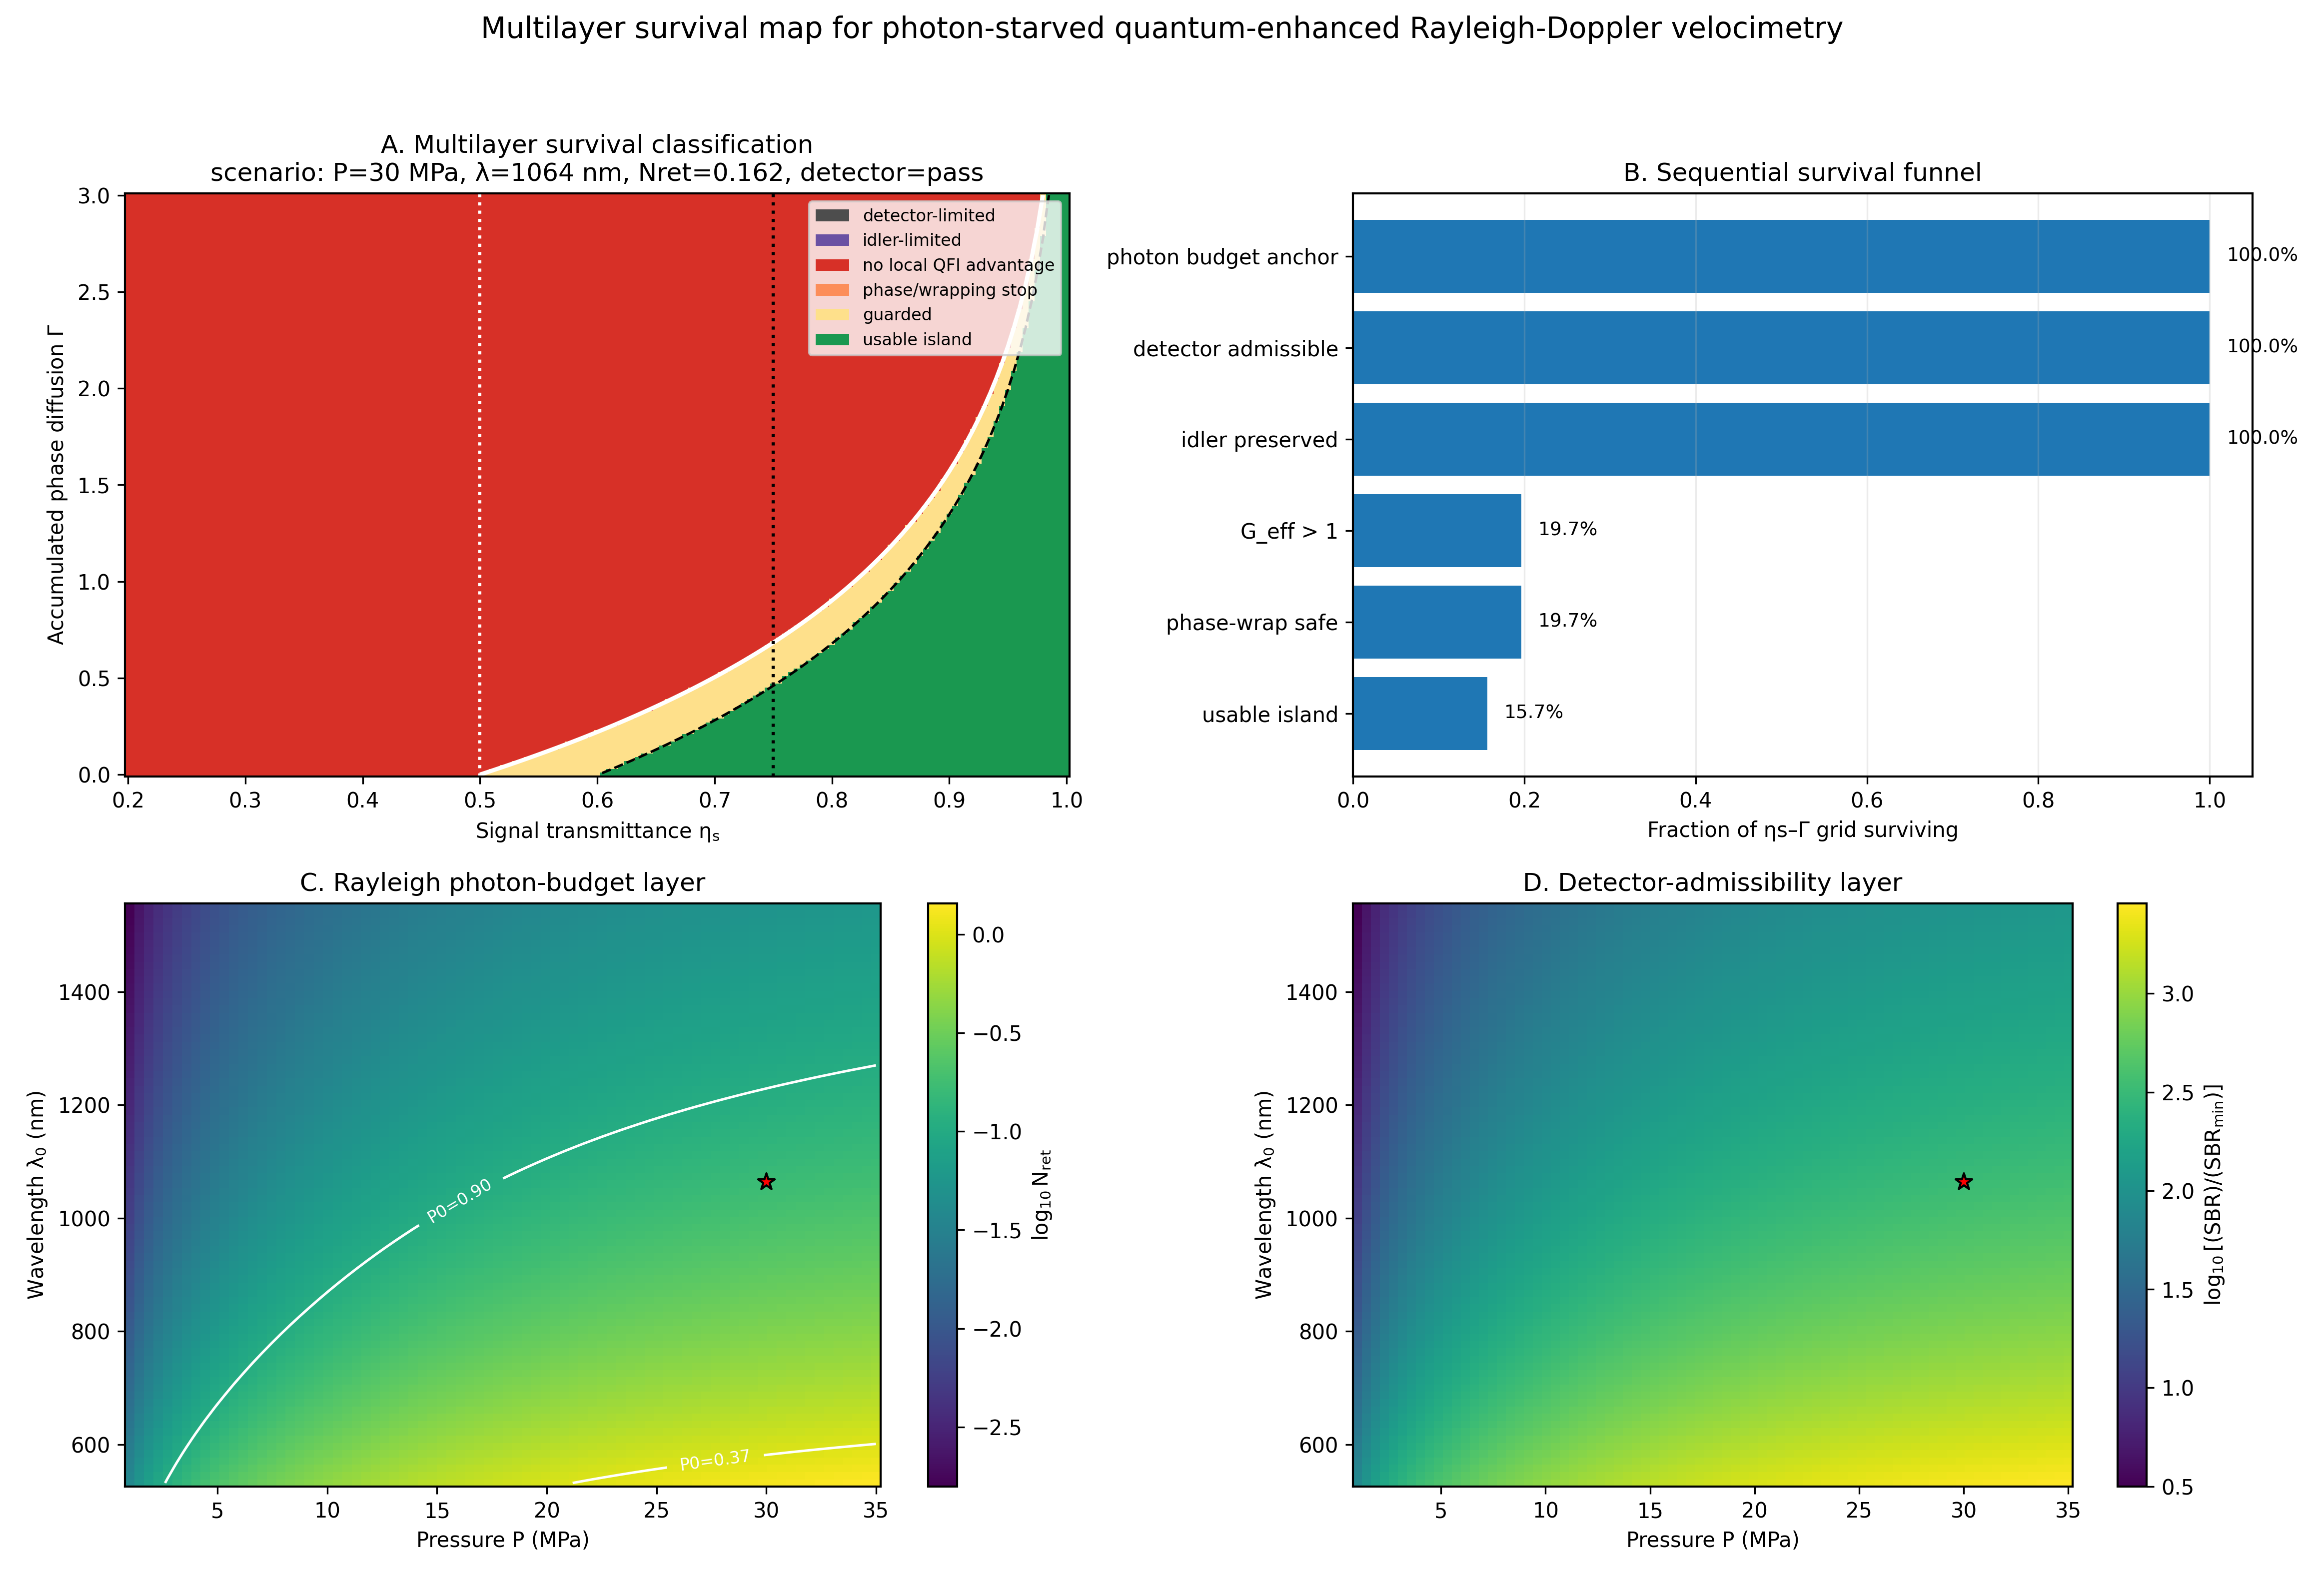
\includegraphics[width=0.98\textwidth]{figures/multilayer_survival_map.png}
  \caption{Multilayer admissibility map. Panel A classifies the $\eta_s$--$\Gamma$ plane after applying detector admissibility, idler preservation, local TMSV advantage, phase-wrapping, and guard-band screens. Panel B shows the sequential screening funnel for the selected Rayleigh budget anchor. Panel C shows the Rayleigh photon-budget layer, and Panel D shows the detector-admissibility margin. This figure is the main synthesis of the paper: an admissible quantum-advantage region remains only after all layers are passed.}
  \label{fig:multilayer}
\end{figure}

\begin{table}[htbp]
\centering
\caption{Scenario-level boundary examples. The table includes pass, guarded, detector-limited, signal-loss-limited, diffusion-limited, and idler-limited cases. The first-failed-layer column makes the multilayer logic explicit.}
\label{tab:scenario_verdicts}
\tiny
\renewcommand{\arraystretch}{1.12}
\begin{tabularx}{\textwidth}{l c c c c c c p{0.15\textwidth}p{0.17\textwidth}X}
\toprule
Case & $P$ & $\lambda_0$ & $\Nret$ & $\etas$ & $\etai$ & $\Gamma$ & Verdict & First failed layer & Reason \\
 & MPa & nm &  &  &  &  &  &  &  \\
\midrule
A & 30 & 532 & 1.30 & 0.90 & 0.90 & 0.50 & local-valid & none & passes configured screens \\
B & 30 & 1064 & 0.163 & 0.90 & 0.90 & 0.50 & local-valid & none & photon-starved but locally interpretable \\
C & 30 & 1550 & 0.0526 & 0.90 & 0.90 & 0.50 & detector-limited & receiver admissibility & SBR or $\Nret$ below detector screen \\
D & 30 & 532 & 1.30 & 0.45 & 0.90 & 0.50 & stop-extrapolation & pure-loss QFI & $\etas<0.5$ and $\Geff\le1$ \\
E & 30 & 532 & 1.30 & 0.90 & 0.90 & 2.00 & stop-extrapolation & phase diffusion & diffusion removes local advantage \\
F & 30 & 532 & 1.30 & 0.90 & 0.50 & 0.50 & idler-limited & idler preservation & idler efficiency below threshold \\
G & 30 & 532 & 1.30 & 0.70 & 0.90 & 0.55 & guarded & global distinguishability & near local boundary; check recommended \\
\bottomrule
\end{tabularx}
\end{table}

The point of Table~\ref{tab:scenario_verdicts} is not to predict a particular field instrument. It demonstrates that a multilayer boundary analysis can produce different verdicts for different failure modes. In particular, $\Nret$ and $\Ns$ remain separated: the table combines a macroscopic Rayleigh budget anchor with assumed microscopic probe/channel parameters rather than identifying the two.

\section{Global validity checks: phase wrapping and finite-dimensional QZZB}
\label{sec:qzzb}

Local QFI is a derivative-based quantity. It can understate global ambiguity when the prior is wide, phase diffusion is strong, or the local phase error approaches the interferometric period. The purpose of the QZZB layer is not to replace the local QFI calculation, but to identify where local variance propagation becomes overly optimistic. In particular, the QZZB module is not used to certify full high-$N_S$ performance; it is used to falsify local-QFI extrapolations whenever finite-prior distinguishability already fails in the finite-dimensional model. This asymmetric role is useful for review: it is stronger at ruling out unsupported local claims than at proving a globally attainable high-photon-number advantage.

Phase wrapping and QZZB play different roles. The wrapping probability is a local-coordinate diagnostic: it asks whether a Gaussian phase-error model is becoming incompatible with the $2\pi$ periodicity of phase. The QZZB is a finite-prior global distinguishability lower bound: it asks whether phase-shifted quantum states remain distinguishable over finite separations. The two checks are therefore complementary rather than redundant.

We use a diagnostic QZZB expression of the form
\begin{equation}
\Sigma_{\mathrm{ZZ}} \ge \frac{1}{2}\int_0^W d\tau\,\tau\left(1-\frac{\tau}{W}\right)
\left[1-\sqrt{1-F(\rho_\phi,\rho_{\phi+\tau})}\right],
\label{eq:qzzb}
\end{equation}
where $W$ is the phase prior width and $F$ denotes the Uhlmann fidelity amplitude under the convention used in the scripts. If a squared-fidelity convention is adopted, the integrand must be modified consistently.

The diagnostic protocol is:
\begin{enumerate}[label=(\alph*)]
  \item construct a truncated two-mode TMSV state in a product Fock basis;
  \item apply signal and idler loss through truncated pure-loss Kraus operators;
  \item apply exact signal-number dephasing according to Eq.~\eqref{eq:number_dephasing};
  \item evaluate the fidelity between phase-shifted density matrices on a finite $\tau$ grid;
  \item integrate Eq.~\eqref{eq:qzzb} over a stated prior width $W$;
  \item compare $\Sigma_{\mathrm{ZZ}}$ with the local surrogate variance and label the point as local-valid, guarded, or stop-extrapolation.
\end{enumerate}
The calculation is finite-dimensional and diagnostic; it is not a high-photon-number global optimality proof. In the main text it is used as a finite-dimensional QZZB check or global distinguishability check.

The guarded phase variance is propagated to projected velocity as
\begin{equation}
  \Var_{\mathrm{guard}}(\hat\phi)=\max[\Var_{\mathrm{sur}}(\hat\phi),\Sigma_{\mathrm{ZZ}}],
  \qquad
  \sigma_v=\frac{\sqrt{\Var_{\mathrm{guard}}}}{K_D\tau_{\mathrm{int}}}.
\end{equation}

\begin{figure}[htbp]
  \centering
  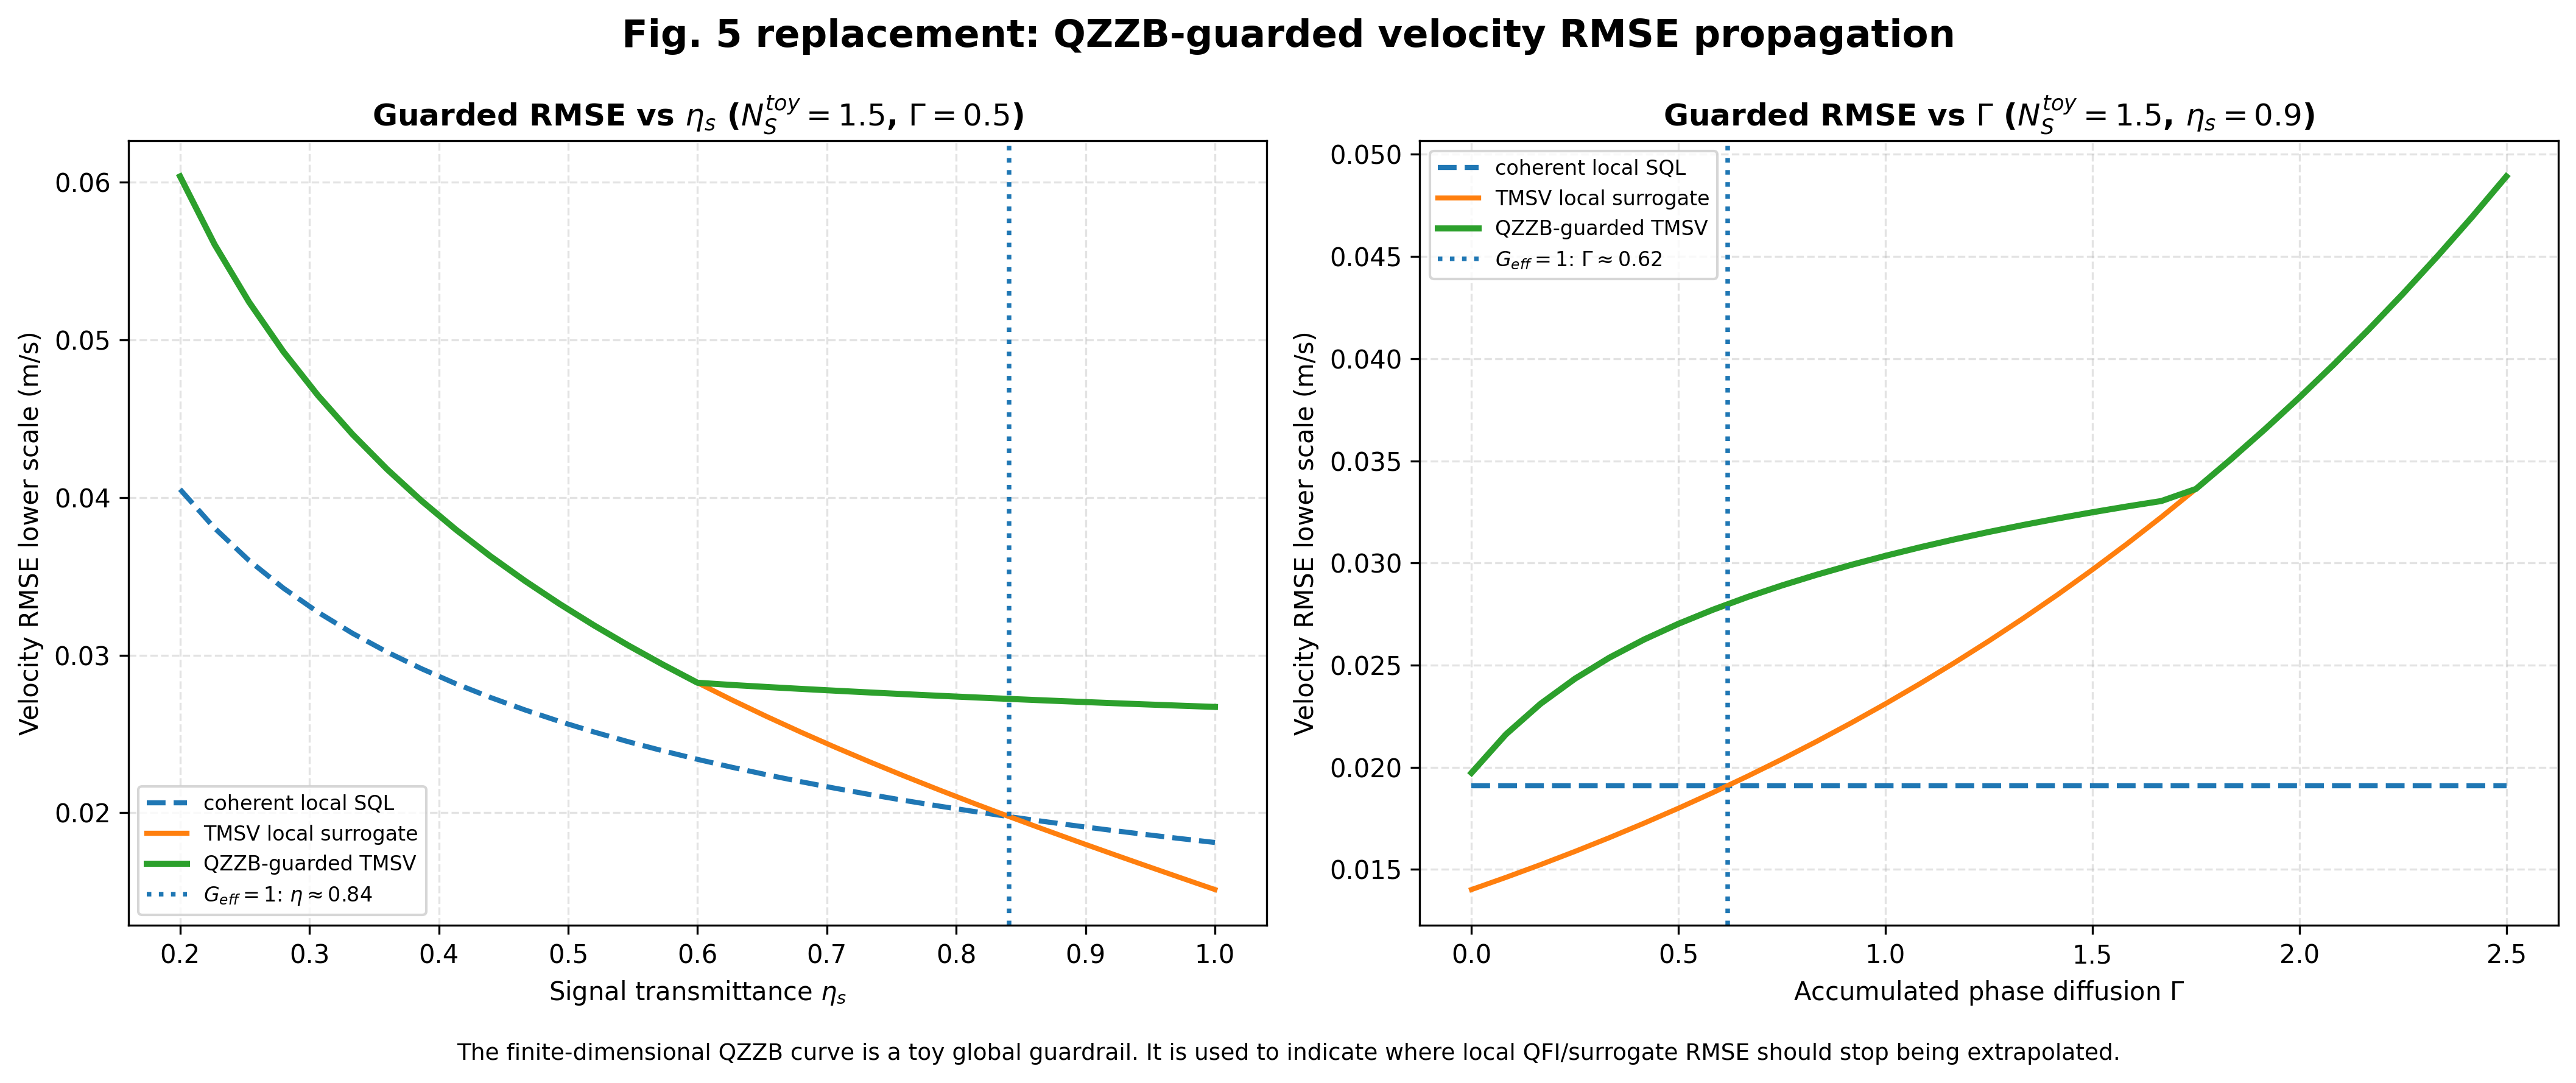
\includegraphics[width=0.88\textwidth]{fig5_qzzb_guarded_rmse.png}
  \caption{QZZB-guarded phase-to-velocity RMSE propagation in a finite-dimensional diagnostic model. The dashed curve is the coherent local SQL, the orange curve is the local TMSV surrogate, and the green curve applies the conservative guard $\max(\Var_{\mathrm{sur}},\Sigma_{\mathrm{ZZ}})$ before mapping phase uncertainty to velocity. The plot is a diagnostic guardrail rather than a full high-photon-number global optimality proof.}
  \label{fig:qzzb_rmse}
\end{figure}

\begin{table}[htbp]
\centering
\caption{Cutoff convergence check for the finite-dimensional diagnostic QZZB check at $N_S^{\mathrm{diag}}=1.5$, $\eta_s=0.9$, $\eta_i=1.0$, and $\Gamma=0.5$. The small drift from $n_{\mathrm{cut}}=10$ to 12 supports the use of the calculation as a qualitative guardrail.}
\label{tab:cutoff}
\begin{tabular}{cccc}
\toprule
$n_{\mathrm{cut}}$ & $N_{S,\mathrm{cut}}$ & $\Sigma_{\mathrm{ZZ}}$ & numerical QFI \\
\midrule
6 & 1.2064 & 0.4152 & 1.1626 \\
8 & 1.3633 & 0.4079 & 1.2138 \\
10 & 1.4392 & 0.4054 & 1.2320 \\
12 & 1.4738 & 0.4044 & 1.2385 \\
\bottomrule
\end{tabular}
\end{table}

\begin{figure}[htbp]
  \centering
  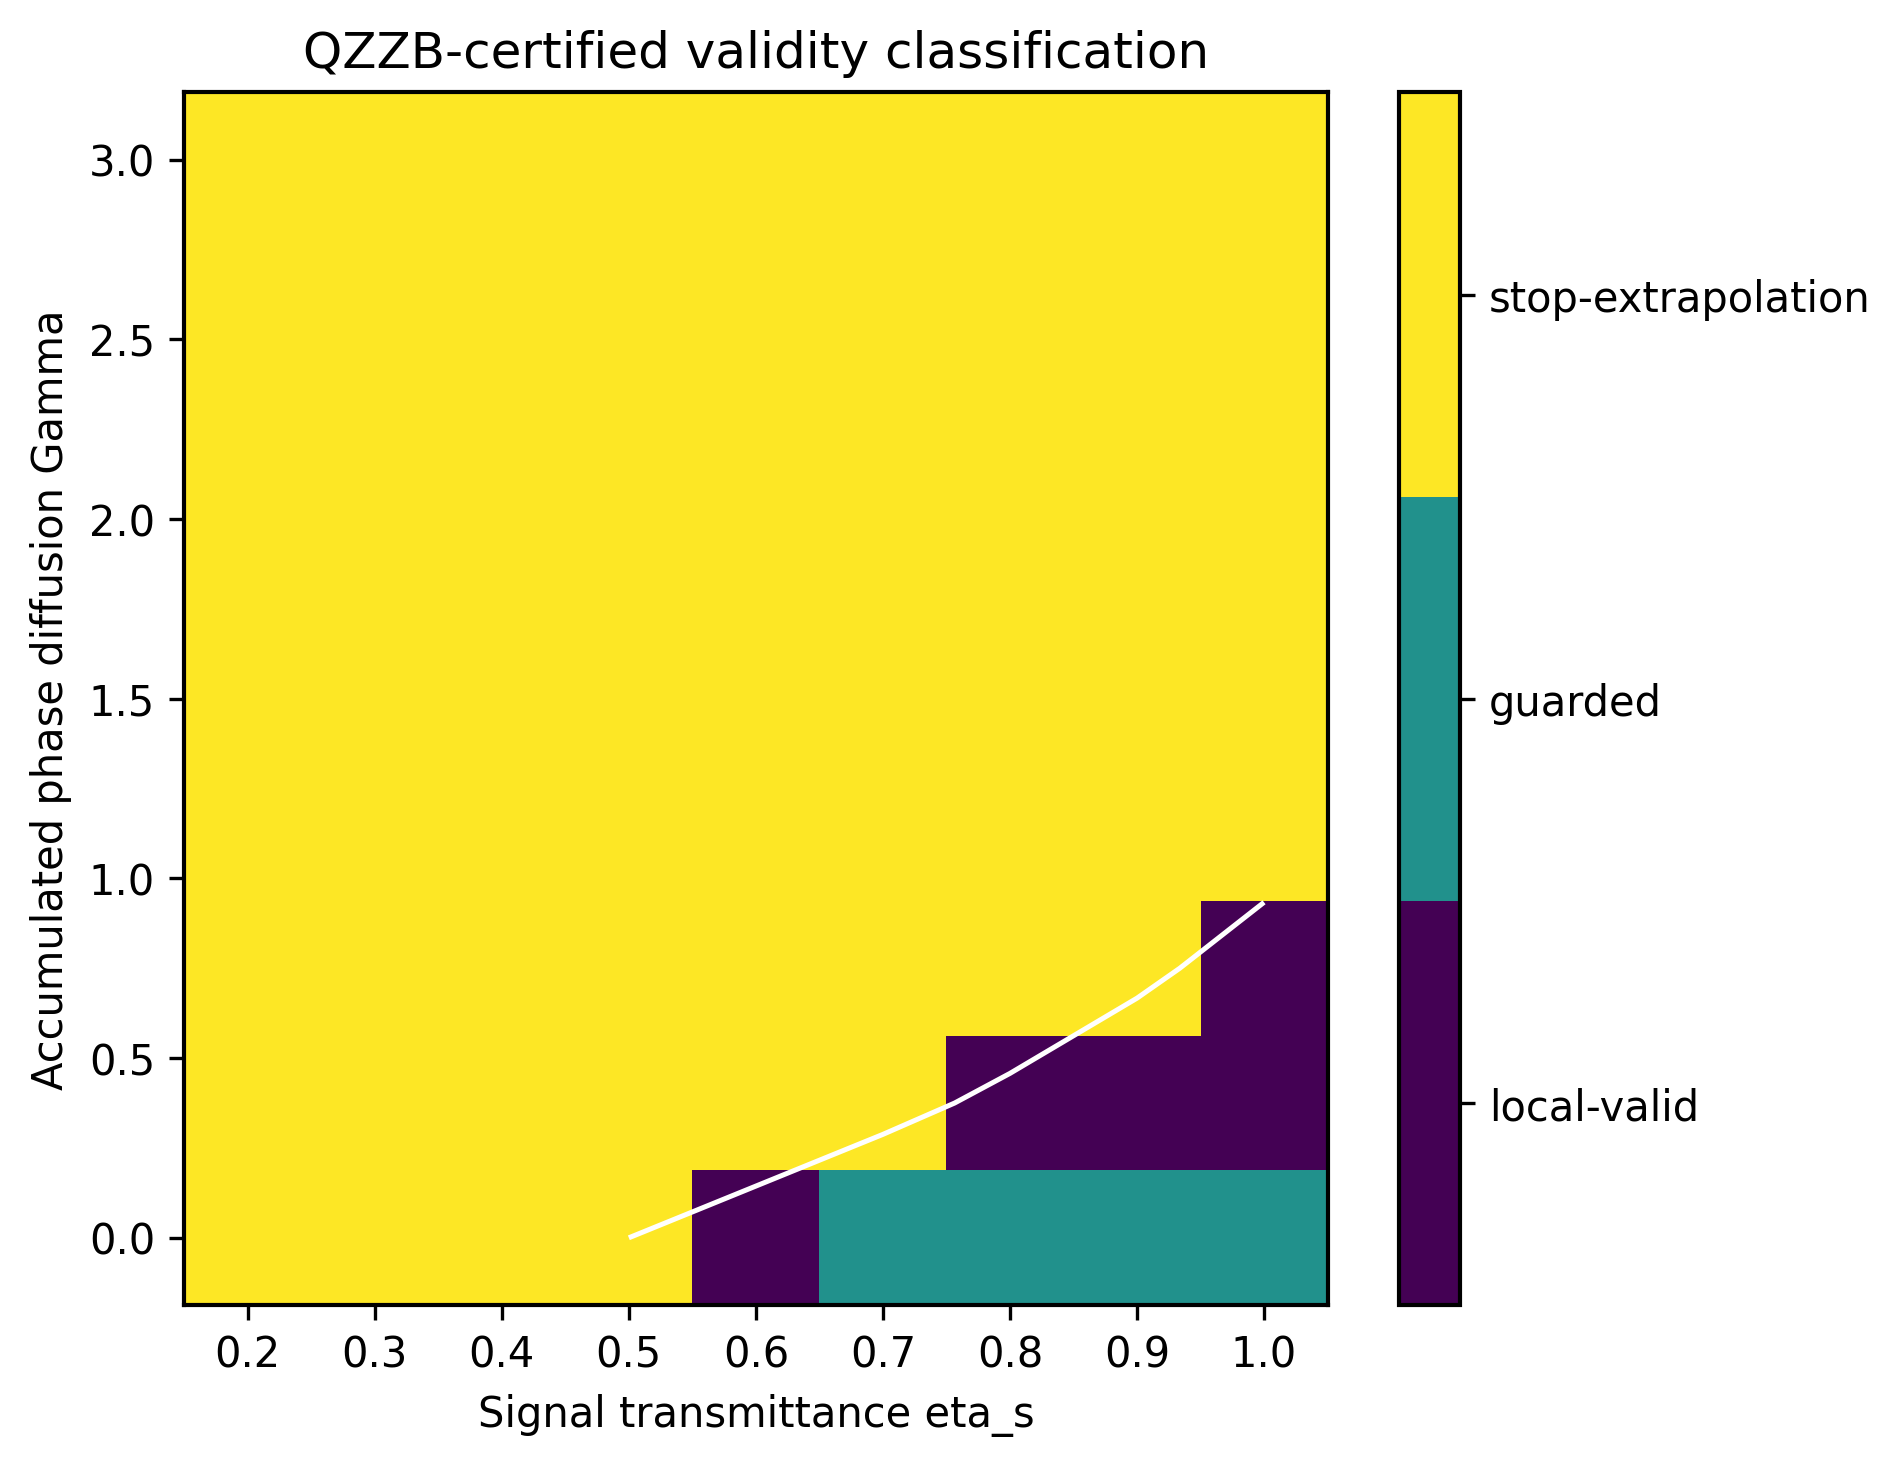
\includegraphics[width=0.82\textwidth]{figures/fig_qzzb_certified_classification.png}
  \caption{QZZB-certified validity classification. The map partitions the local model into local-valid, guarded, and stop-extrapolation regions using the analytic local boundary, QZZB guard ratio, and phase-wrapping risk. It marks where the local model is locally valid, guarded, or stopped by the configured tests.}
  \label{fig:qzzb_classification}
\end{figure}

\section{Idler-loss sensitivity as a second survival condition}
\label{sec:idler}

The analytic one-sided-loss formula in Proposition~1 assumes ideal idler preservation. This assumption is not innocuous. In an actual TMSV protocol the idler must be stored, transported, mode-matched, and detected well enough to retain the signal--idler correlations that generated the QFI advantage. We therefore treat idler efficiency $\etai$ as a second survival condition.

The finite-dimensional QFI scan repeats the calculation over both $\etas$ and $\etai$. Poor idler preservation suppresses the TMSV advantage even when signal transmittance is moderate. Thus satisfying $\etas>0.5$ under the equal-signal-energy convention is not sufficient: the idler path must also preserve enough correlation to keep the TMSV/coherent QFI ratio above unity.

\begin{figure}[htbp]
  \centering
  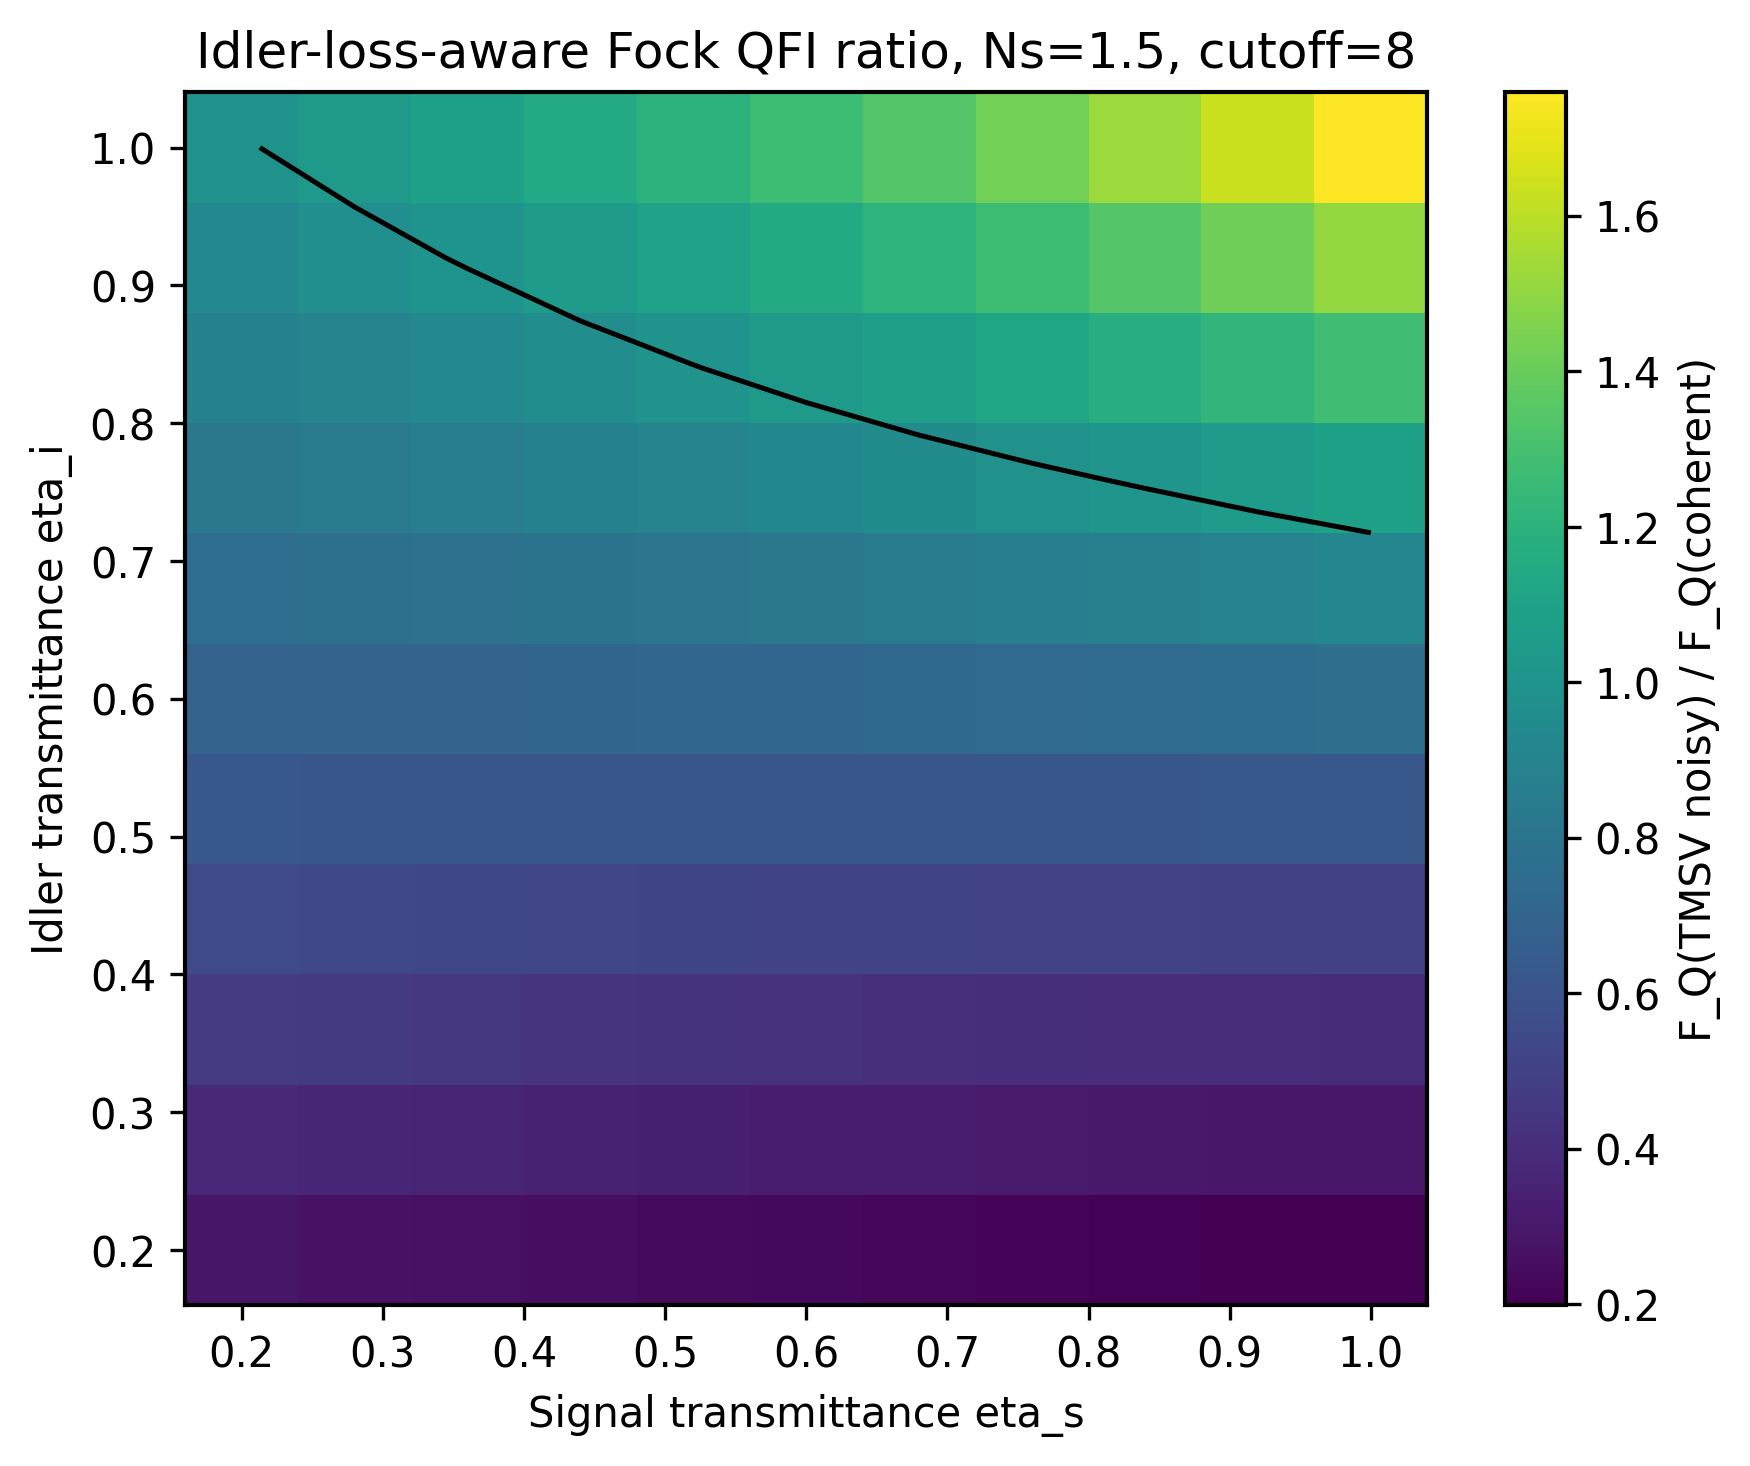
\includegraphics[width=0.74\textwidth]{figures/fig_idler_loss_fock_qfi_ratio.png}
  \caption{Idler-loss-aware finite-dimensional QFI ratio. The color scale shows the TMSV/coherent QFI ratio as a function of signal transmittance and idler efficiency. The $G=1$ contour indicates where idler imperfection removes the TMSV advantage. Idler preservation is therefore a second survival condition rather than a minor implementation detail.}
  \label{fig:idler_loss}
\end{figure}

\section{Falsifiable red lines for future experiments}
\label{sec:redlines}

The boundary analysis can be compressed into falsifiable checks that future simulations or experiments can attempt to violate.
\begin{enumerate}[label=(\alph*)]
  \item Under equal signal-mode energy and one-sided pure loss, a local TMSV QFI advantage requires $\etas>1/2$.
  \item Under equal total source energy, the conservative pure-loss boundary is $\eta_c^{\mathrm{tot}}=3/4+1/(4\Ns)$, approaching $0.75$ for large $\Ns$.
  \item Under the first-order loss--diffusion envelope, local advantage requires $\Gamma<\ln \GQ(\etas,\Ns)$.
  \item If $\GQ\le1$, no choice of the phase-diffusion exponent convention in $\GQ e^{-a\Gamma}$ can recover a local TMSV advantage.
  \item When phase-wrapping contours approach or cross the $\Geff=1$ boundary, local QFI/RMSE propagation should not be interpreted as attainable performance without a global guardrail.
  \item Even when $\Geff>1$, a point is detector-inadmissible if $\Nret/N_{\mathrm{noise}}<\SBR_{\min}$ or $\Nret<N_{\mathrm{noise}}$.
  \item Even when the signal path passes the pure-loss threshold, insufficient idler preservation can remove the TMSV advantage.
\end{enumerate}
These red lines are more important than any single favorable numerical point. They define what would falsify a claimed photon-starved quantum advantage in this framework.

\section{Responsible interpretation, limitations, and transferability}
\label{sec:limitations}

This work is a multilayer boundary study rather than a field-deployed quantum velocimeter. It does not claim a demonstrated industrial quantum advantage, a complete high-photon-number QZZB solution, a detector-specific POVM model, or a validated pipeline-flow reconstruction. The role of the paper is to identify where a TMSV-based local advantage can remain interpretable and where that interpretation should be stopped. The phase-diffusion model is an effective surrogate motivated by refractive-index wandering and number dephasing; the QZZB calculations are finite-dimensional tests of global distinguishability; detector admissibility is a receiver-layer screen.

GERG-2008, Lorentz--Lorenz refractivity corrections, and sparse-field assimilation provide possible future interfaces for propagating local velocity uncertainty into a macroscopic uncertainty budget \cite{KunzWagner2012,Lorentz1880,Lorenz1880,JCGM2008,Evensen2003}. They are not treated as completed thermodynamic compensation, CFD/EnKF reconstruction, or industrial validation. Appendix~\ref{app:detector_macro} gives an illustrative 1D uncertainty-transfer example only to show how a reduced local velocity variance would enter a downstream uncertainty band.

Beyond the specific Rayleigh--Doppler setting considered here, the framework illustrates a general requirement for weak-return quantum sensing in open systems: a claimed local quantum advantage must survive not only loss, but also dephasing, idler degradation, detector admissibility, and global distinguishability checks. Similar survival-boundary questions may arise in quantum illumination/LIDAR under turbulent or lossy channels and in non-invasive scattering measurements in lossy media. The numerical results here are not directly transferable to those platforms without rebuilding the photon budget, noise model, and detection statistics.

\section{Conclusion}

This paper establishes a multilayer admissibility analysis for quantum-enhanced Rayleigh--Doppler velocimetry in photon-starved high-pressure gases. The first boundary is the Rayleigh photon budget: $\Nret$ and the zero-count probability determine whether a low-return window exists. The second boundary is detector admissibility: dark/background counts and gate time decide whether that low-return point remains experimentally measurable. The third boundary is pure-loss TMSV QFI: under equal signal-mode energy the survival threshold is $\etas=1/2$, while the equal-total-source-energy threshold approaches $\etas\simeq0.75$. The fourth boundary is loss--diffusion survival: accumulated phase diffusion must satisfy $\Gamma<\ln\GQ$. The fifth boundary is global validity: phase wrapping and finite-dimensional QZZB checks decide whether local variance propagation can still be interpreted. The sixth boundary is idler preservation: the retained idler must remain sufficiently efficient for the TMSV correlation to be useful.

The resulting message is not that quantum-enhanced velocimetry is generically superior in industrial gas measurements. Rather, an admissible advantage region exists only if the optical, detector, quantum-channel, idler, and global-estimation screens are all passed. This shifts the claim from an unconditional quantum advantage to a falsifiable multilayer map. The public reproduction package provides the numerical scripts, configuration files, tests, processed tables, and figure-generation workflow needed to check the photon budget, QFI boundary, diffusion envelope, QZZB checks, detector screen, idler-loss map, and scenario verdicts.

\section*{Data and code availability}
The code and processed data supporting the numerical results in this work are available at: \repoURL. The repository contains the scripts used to generate the Rayleigh photon-budget maps, SQL baselines, TMSV QFI advantage diagrams, loss--diffusion survival islands, multilayer admissibility maps, QZZB-guarded RMSE curves, QZZB-certified validity diagrams, idler-loss sensitivity maps, detector-level admissibility scans, illustrative uncertainty-transfer examples, and scenario-level boundary tables. The manuscript source files are not included in the public repository.

\section*{Funding}
No external funding is reported for the numerical work described in this manuscript.

\appendix

\section{Notation, covariance convention, and resource accounting}
\label{app:notation}

For a continuous-variable system with $m$ bosonic modes, define the quadrature vector
\begin{equation}
  \hat R=(\hat x_1,\hat p_1,\hat x_2,\hat p_2,\ldots,\hat x_m,\hat p_m)^T.
\end{equation}
The canonical commutation relation is $[\hat R_j,\hat R_k]=i\Omega_{jk}$. We use the $\hbar=2$ covariance convention, so the vacuum covariance matrix is the identity matrix. For a zero-mean Gaussian state,
\begin{equation}
  V_{jk}=\frac{1}{2}\langle \Delta \hat R_j\Delta \hat R_k+\Delta \hat R_k\Delta \hat R_j\rangle.
\end{equation}
The physicality condition is $V+i\Omega\ge0$.

The manuscript uses two resource-accounting criteria. The default criterion is equal signal-mode energy: the coherent state and the TMSV signal mode each use $\Ns$ signal photons. This criterion isolates the effect of the retained idler correlations. The conservative check is equal total source energy: the coherent state is allowed the signal-plus-idler energy used by TMSV. This doubles the coherent-state benchmark and shifts the pure-loss threshold from $\etas=0.5$ to $\eta_c^{\mathrm{tot}}=3/4+1/(4\Ns)$.

\section{Pure-loss TMSV QFI derivation}
\label{app:qfi}

The ideal TMSV covariance matrix is
\begin{equation}
V_0=\begin{pmatrix}
(2\Ns+1)I_2 & 2\sqrt{\Ns(\Ns+1)}Z_2\\
2\sqrt{\Ns(\Ns+1)}Z_2 & (2\Ns+1)I_2
\end{pmatrix}.
\end{equation}
A one-sided vacuum pure-loss channel acting on the signal mode maps it to
\begin{equation}
V_\eta=(K\oplus I_2)V_0(K\oplus I_2)^T+[(1-\eta)I_2]\oplus 0_2,
\qquad K=\sqrt{\eta}I_2.
\end{equation}
Equivalently,
\begin{equation}
V_\eta=\begin{pmatrix}
[1+2\eta\Ns]I_2 & 2\sqrt{\eta\Ns(\Ns+1)}Z_2\\
2\sqrt{\eta\Ns(\Ns+1)}Z_2 & (2\Ns+1)I_2
\end{pmatrix}.
\end{equation}
The signal phase is encoded as $V_\eta(\phi)=R_\phi V_\eta R_\phi^T$ with $R_\phi=\exp(\phi J_2)\oplus I_2$. The covariance derivative at $\phi=0$ is
\begin{equation}
  \dot V_\eta=(J_2\oplus0_2)V_\eta+V_\eta(J_2^T\oplus0_2).
\end{equation}
Substitution into the zero-displacement Gaussian-state QFI moment formula gives Eq.~\eqref{eq:tmsv_qfi}. Table~\ref{tab:qfi_audit} lists the minimum consistency checks.

\begin{table}[htbp]
\centering
\caption{Audit checklist for the pure-loss TMSV QFI derivation.}
\label{tab:qfi_audit}
\small
\begin{tabularx}{\textwidth}{l X}
\toprule
Item & Required check \\
\midrule
Phase carrier & $\phi$ acts only on the signal-mode quadratures through $R_\phi\oplus I_2$. \\
Loss model & Vacuum pure-loss channel is applied to the signal mode with $K=\sqrt{\eta}I_2$. \\
Idler treatment & Idler covariance block remains $(2\Ns+1)I_2$ in the first-order analytic model. \\
Covariance derivative & $\dot V_\eta=(J_2\oplus0_2)V_\eta+V_\eta(J_2^T\oplus0_2)$. \\
Limiting check & At $\eta=1$, $F_Q=4\Ns(\Ns+1)$, recovering the lossless TMSV phase-estimation scaling. \\
Resource check & Equal-total-source-energy comparison doubles the coherent-state benchmark. \\
\bottomrule
\end{tabularx}
\end{table}

For $\Ns=100$, representative advantage ratios are $\GQ(0.90,100)=4.8095$, $\GQ(0.65,100)=1.4225$, $\GQ(0.50,100)=1.0000$, and $\GQ(0.30,100)=0.7163$. These anchors are used in the code tests.

\section{Phase-diffusion surrogate and exponent sensitivity}
\label{app:diffusion}

The phase-diffusion surrogate is a boundary proxy. It starts from number dephasing, which suppresses off-diagonal number-basis elements according to Eq.~\eqref{eq:number_dephasing}. A strict non-Gaussian global QFI calculation under this channel would require a separate analysis. Instead, the envelope
\begin{equation}
  \Geff^{(a)}=\GQ e^{-a\Gamma},\qquad a\in\{1/2,1,2\},
\end{equation}
provides optimistic, baseline, and conservative diffusion screening. The corresponding boundary is
\begin{equation}
  \Gamma_{\max}^{(a)}=\frac{\ln\GQ}{a},\qquad \GQ>1.
\end{equation}
Changing $a$ changes the width of the island, not the topology: if loss already drives $\GQ\le1$, diffusion cannot recover advantage; if $\GQ>1$, increasing $\Gamma$ eventually removes it.

\begin{table}[htbp]
\centering
\caption{Finite-dimensional exact dephasing-QFI sanity checks. The exact Fock-space QFI ratio is not expected to equal the envelope value; the check is used only to verify the monotonic survival trend and the absence of advantage recovery below the pure-loss boundary. Values use a diagnostic cutoff $n_{\mathrm{cut}}=10$.}
\label{tab:dephasing_sanity}
\scriptsize
\begin{tabular}{cccccccl}
\toprule
$N_S^{\mathrm{diag}}$ & $\eta_s$ & $\eta_i$ & $\Gamma$ & exact QFI/coherent & envelope $G_Qe^{-\Gamma}$ & Trend & Verdict \\
\midrule
1.5 & 0.90 & 1.00 & 0.20 & 0.466 & 1.574 & decreasing & local trend survives in envelope \\
1.5 & 0.90 & 1.00 & 0.80 & 0.148 & 0.864 & decreasing & diffusion suppresses advantage \\
1.5 & 0.70 & 1.00 & 0.50 & 0.259 & 0.798 & near boundary & guarded / no strong claim \\
1.5 & 0.50 & 1.00 & 0.20 & 0.550 & 0.819 & no recovery & pure-loss boundary not rescued \\
1.5 & 0.90 & 0.70 & 0.50 & 0.192 & 1.166 & idler-degraded & idler loss suppresses exact QFI \\
\bottomrule
\end{tabular}
\end{table}

\begin{figure}[htbp]
  \centering
  
\includegraphics[width=0.88\textwidth]{figures/fig_phase_diffusion_envelope.png}
  \caption{Phase-diffusion uncertainty envelope for different exponent coefficients $a$. The plot shows how the numerical width of the survival boundary changes while preserving the qualitative loss--diffusion topology.}
\end{figure}

\section{QZZB protocol, cutoff convergence, and diagnostic scaling}
\label{app:qzzb}

The QZZB module constructs a truncated TMSV state
\begin{equation}
  |\psi\rangle=\sum_{n=0}^{n_{\mathrm{cut}}-1}\sqrt{(1-\lambda)\lambda^n}|n,n\rangle,
  \qquad \lambda=\frac{\Ns}{\Ns+1},
\end{equation}
with renormalization after truncation. Signal and idler loss are applied with finite-dimensional pure-loss Kraus operators. Signal-number dephasing is applied exactly within the truncated basis. Phase shifts are generated by $\exp(-i\tau\hat n_s)$, and Uhlmann fidelities between $\rho_\phi$ and $\rho_{\phi+\tau}$ are evaluated before numerical integration of Eq.~\eqref{eq:qzzb}.

\begin{figure}[htbp]
  \centering
  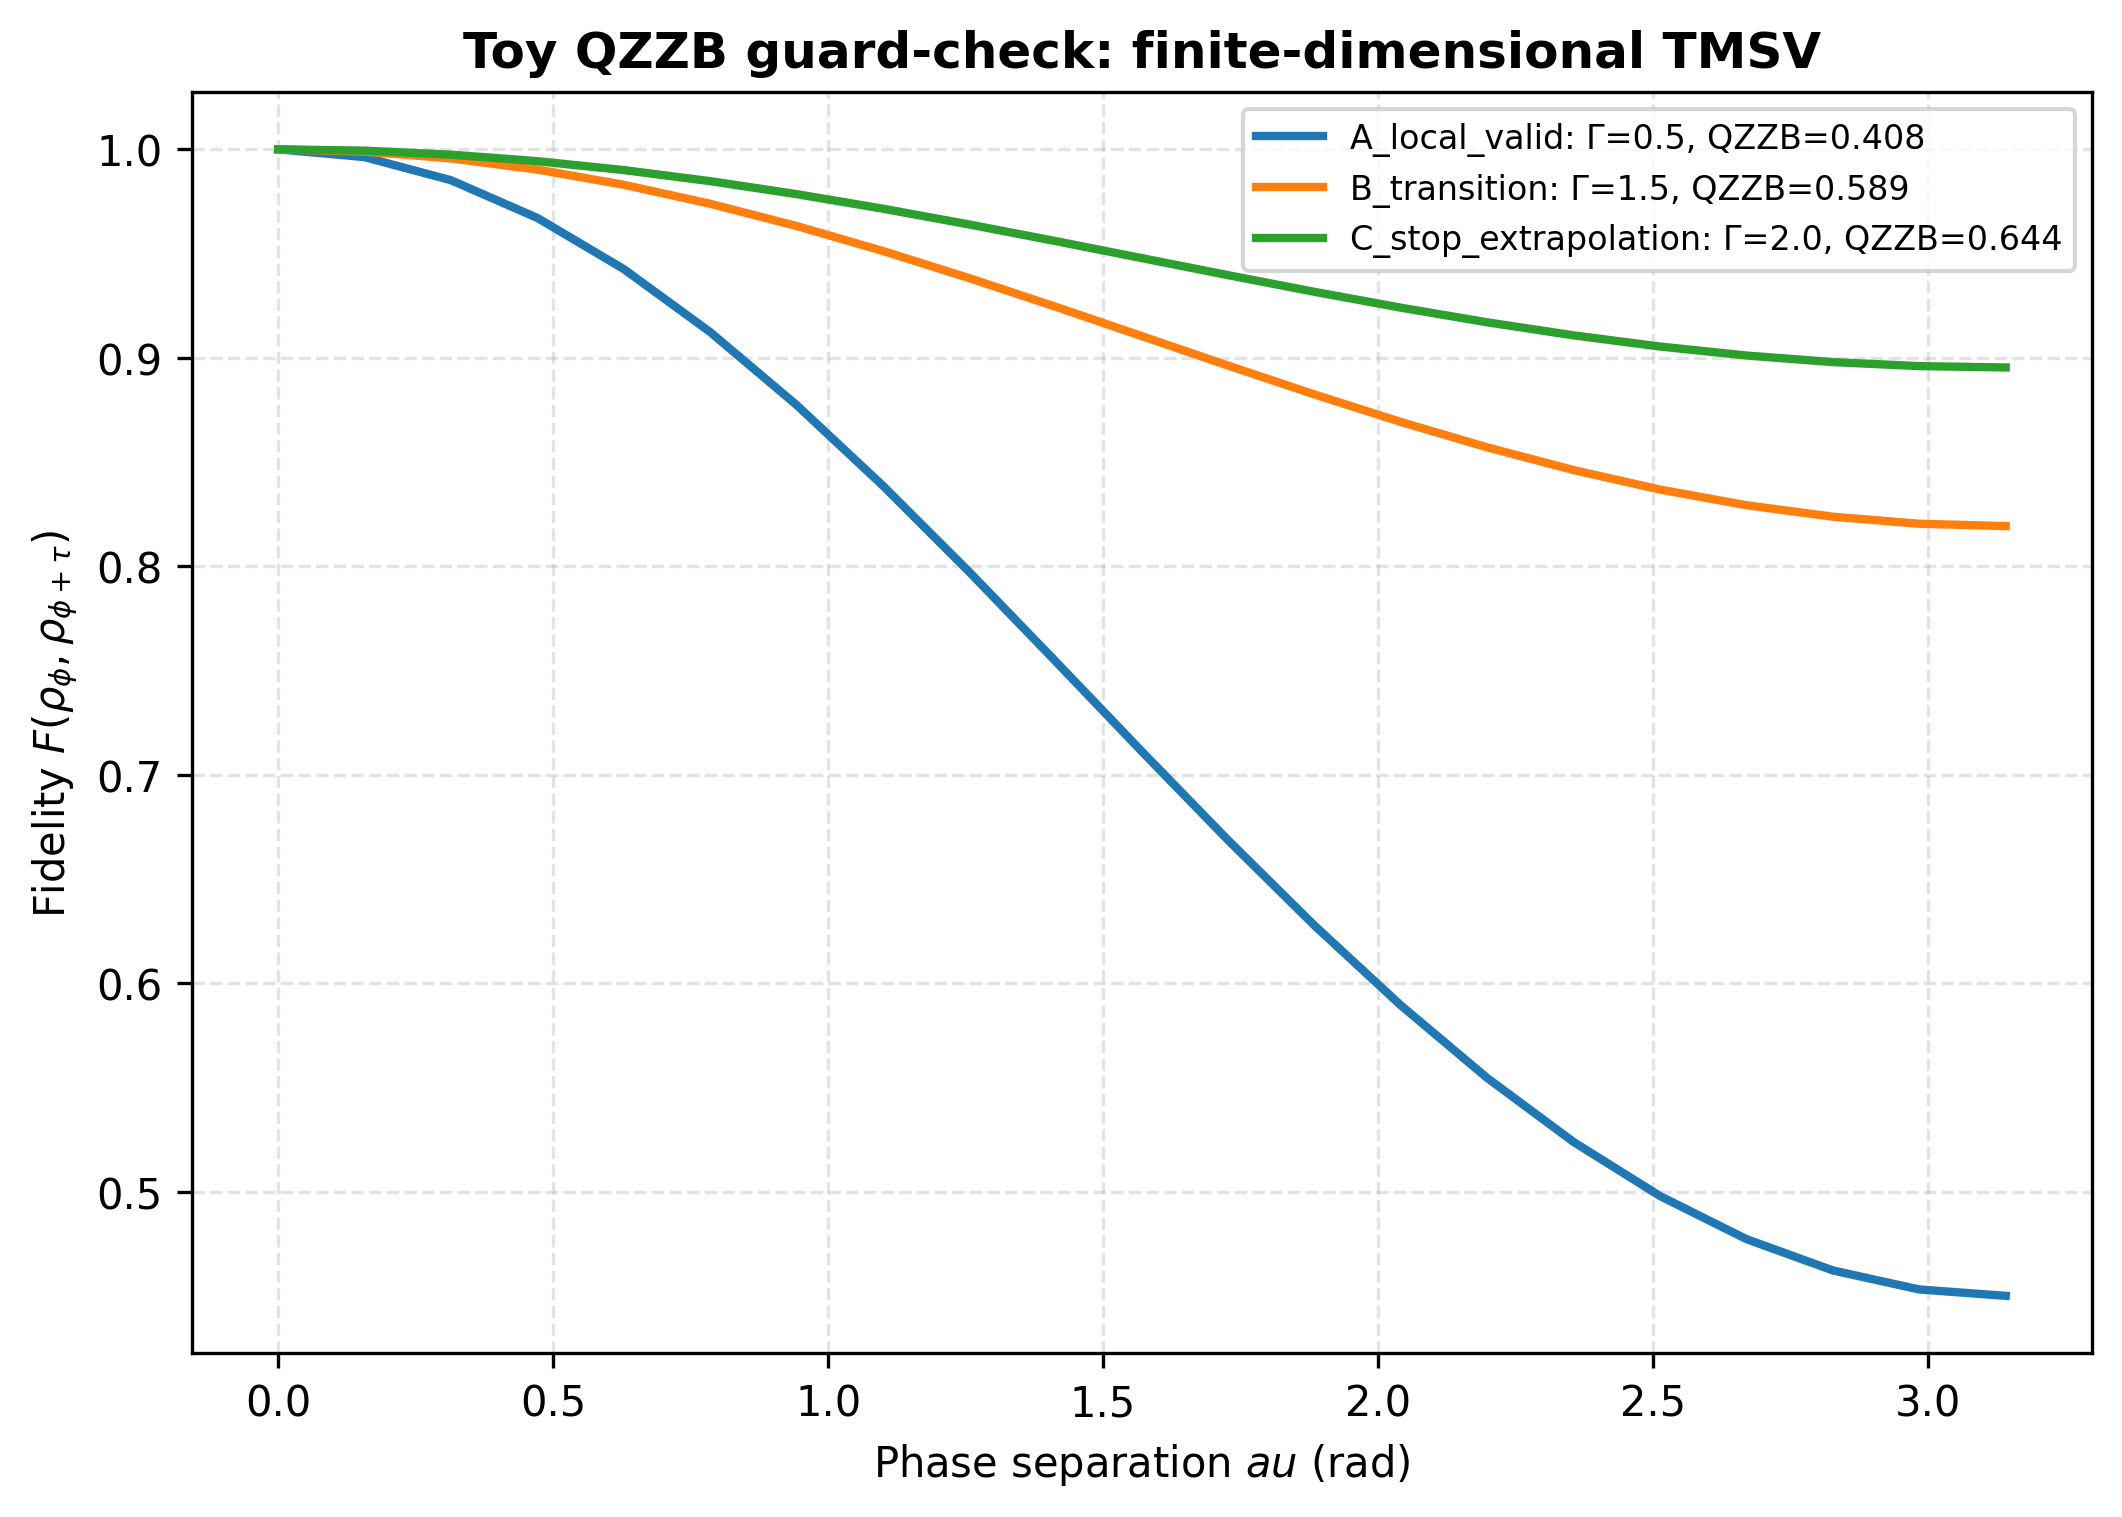
\includegraphics[width=0.78\textwidth]{qzzb_diagnostic_guardcheck_fidelity.png}
  \caption{Finite-dimensional diagnostic QZZB fidelity curves. Stronger accumulated diffusion keeps neighboring phase-shifted states less distinguishable over a wider separation, raising the QZZB lower bound.}
\end{figure}

\begin{figure}[htbp]
  \centering
  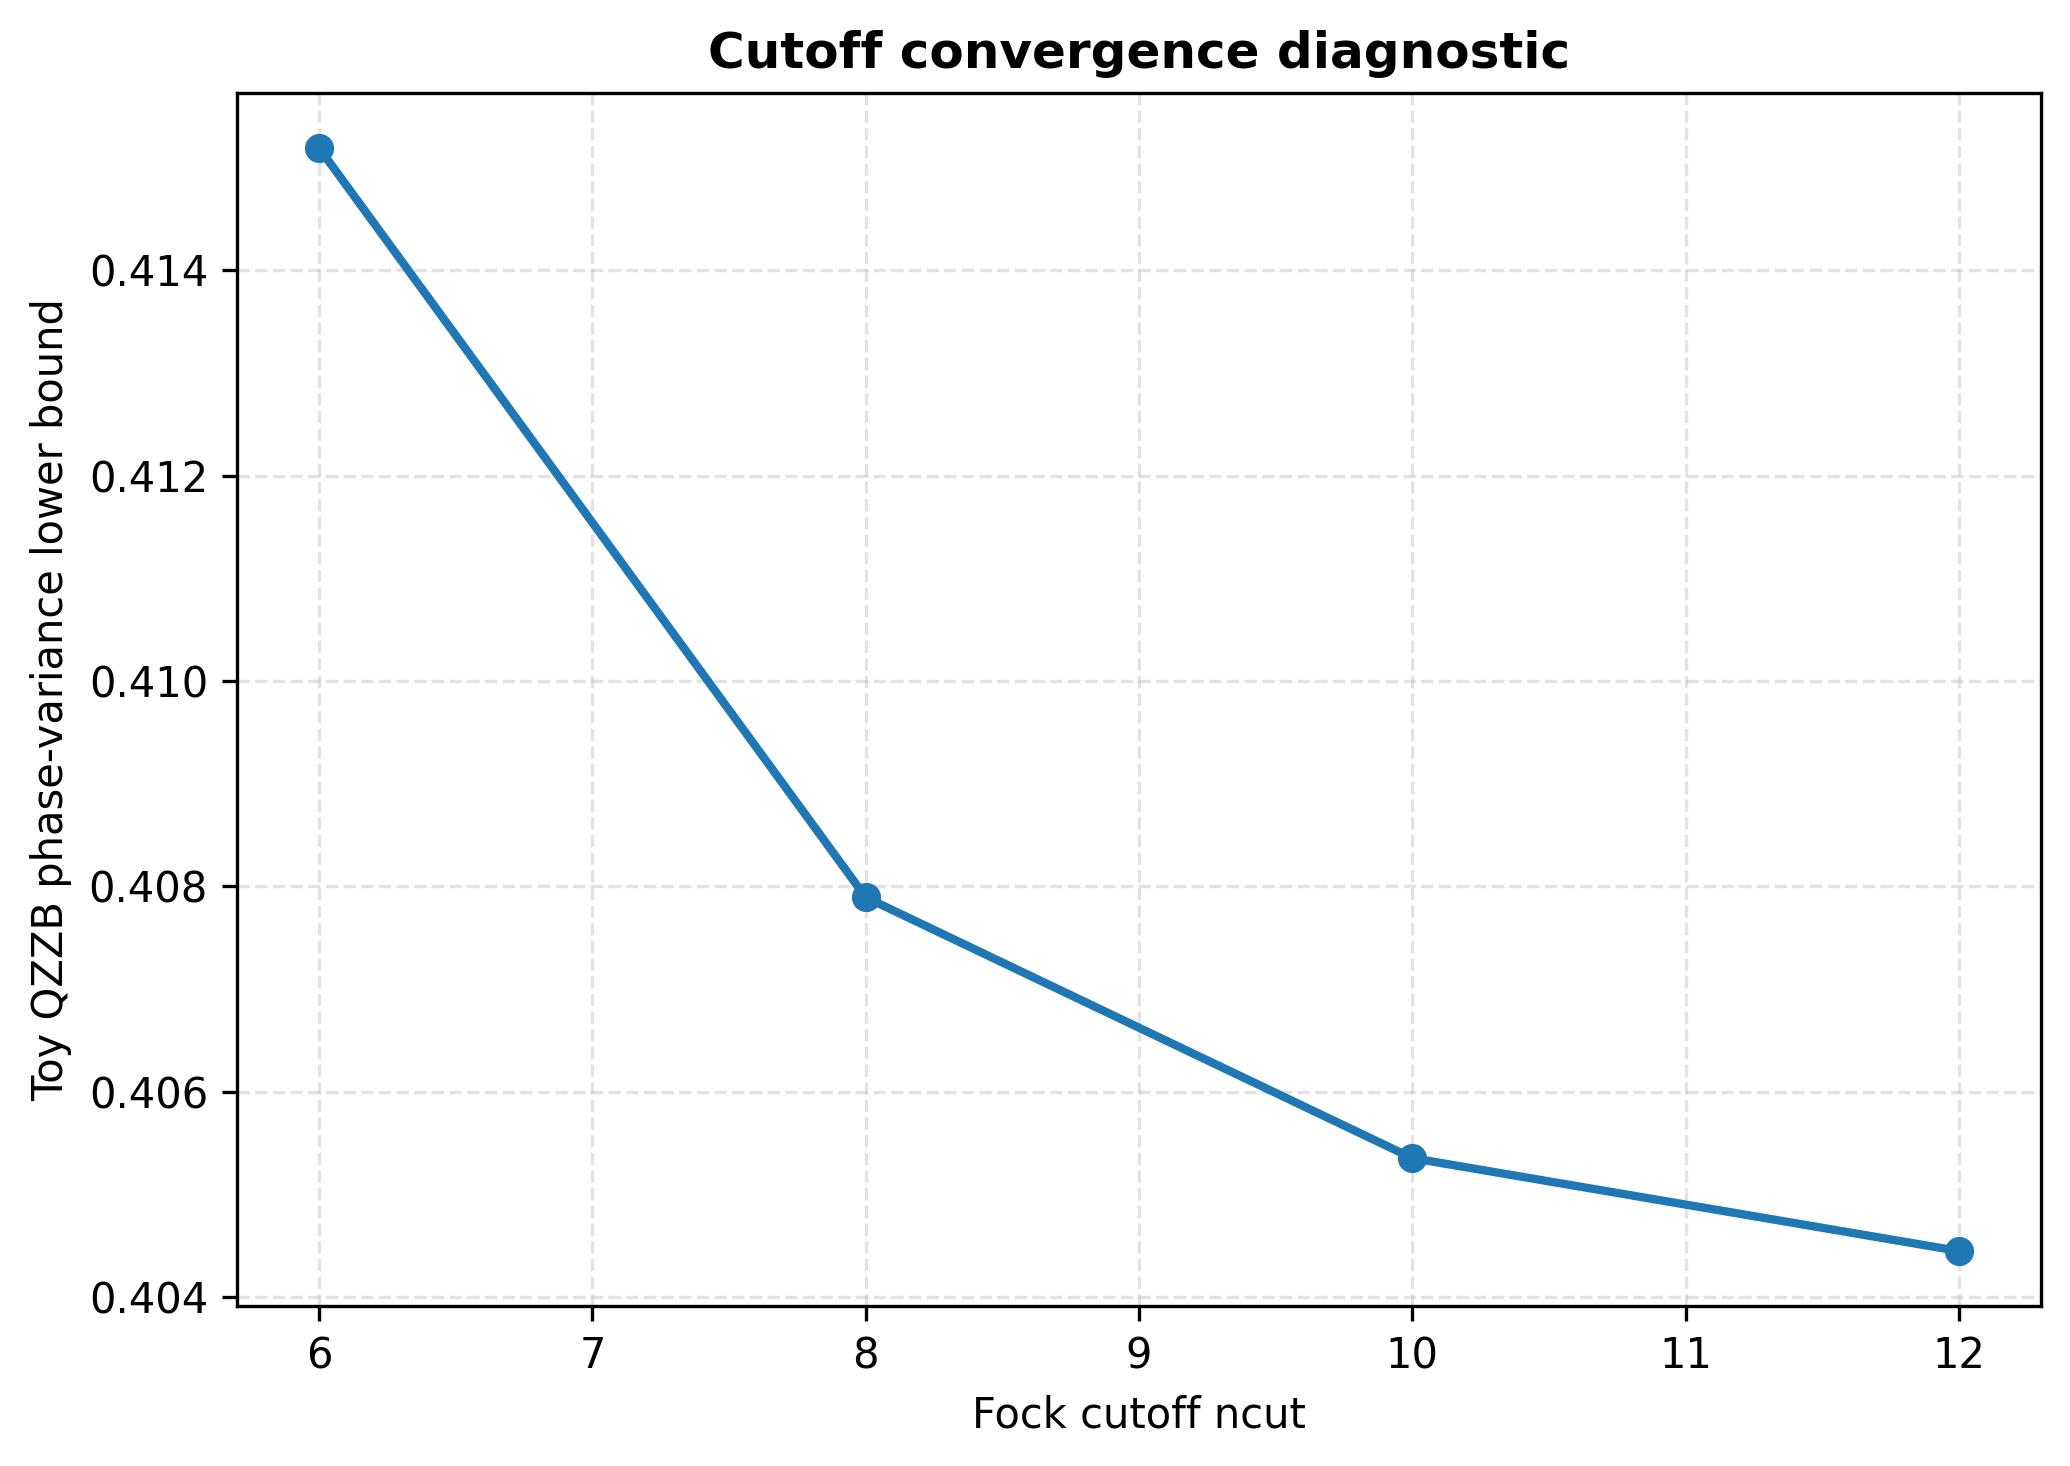
\includegraphics[width=0.72\textwidth]{cutoff_convergence_qzzb.png}
  \caption{Cutoff convergence diagnostic for the finite-dimensional QZZB lower bound. The small change from $n_{\mathrm{cut}}=10$ to 12 indicates that the calculation is stable enough for its intended guardrail role.}
\end{figure}

\begin{table}[htbp]
\centering
\caption{Representative diagnostic QZZB sensitivity checks. The entries are used to check qualitative classification stability under cutoff, prior-width, and noise changes; they are not high-photon-number optimality certificates.}
\label{tab:qzzb_sensitivity}
\scriptsize
\begin{tabular}{ccccccc}
\toprule
Case & $N_S^{\mathrm{diag}}$ & $n_{\mathrm{cut}}$ & $W$ & $(\eta_s,\Gamma)$ & $R_{\mathrm{guard}}$ trend & Class \\
\midrule
A & 1.5 & 8 & $\pi$ & (0.90, 0.30) & low-to-moderate & local-valid / guarded \\
B & 1.5 & 10 & $\pi$ & (0.90, 0.50) & moderate & guarded \\
C & 1.5 & 12 & $\pi$ & (0.90, 0.50) & similar to B & guarded \\
D & 1.5 & 10 & $2\pi$ & (0.90, 0.50) & higher prior penalty & guarded \\
E & 1.5 & 10 & $\pi$ & (0.60, 1.00) & high or no local island & stop-extrapolation \\
F & 1.5 & 10 & $\pi$ & (0.90, 2.00) & high diffusion floor & stop-extrapolation \\
\bottomrule
\end{tabular}
\end{table}

The diagnostic calculation also includes a photon-number scaling guardrail. Low-dimensional QZZB calculations at $N_S^{\mathrm{diag}}\approx1.5$ do not replace high-$\Ns$ global optimality. They indicate how global distinguishability degrades under loss and diffusion. For larger photon number, number-dephasing terms suppress higher-order coherences more strongly, so the low-dimensional guardrail should be read as a conservative check of where local interpretations begin to fail rather than as a proof of attainable high-$\Ns$ RMSE.

\begin{figure}[htbp]
  \centering
  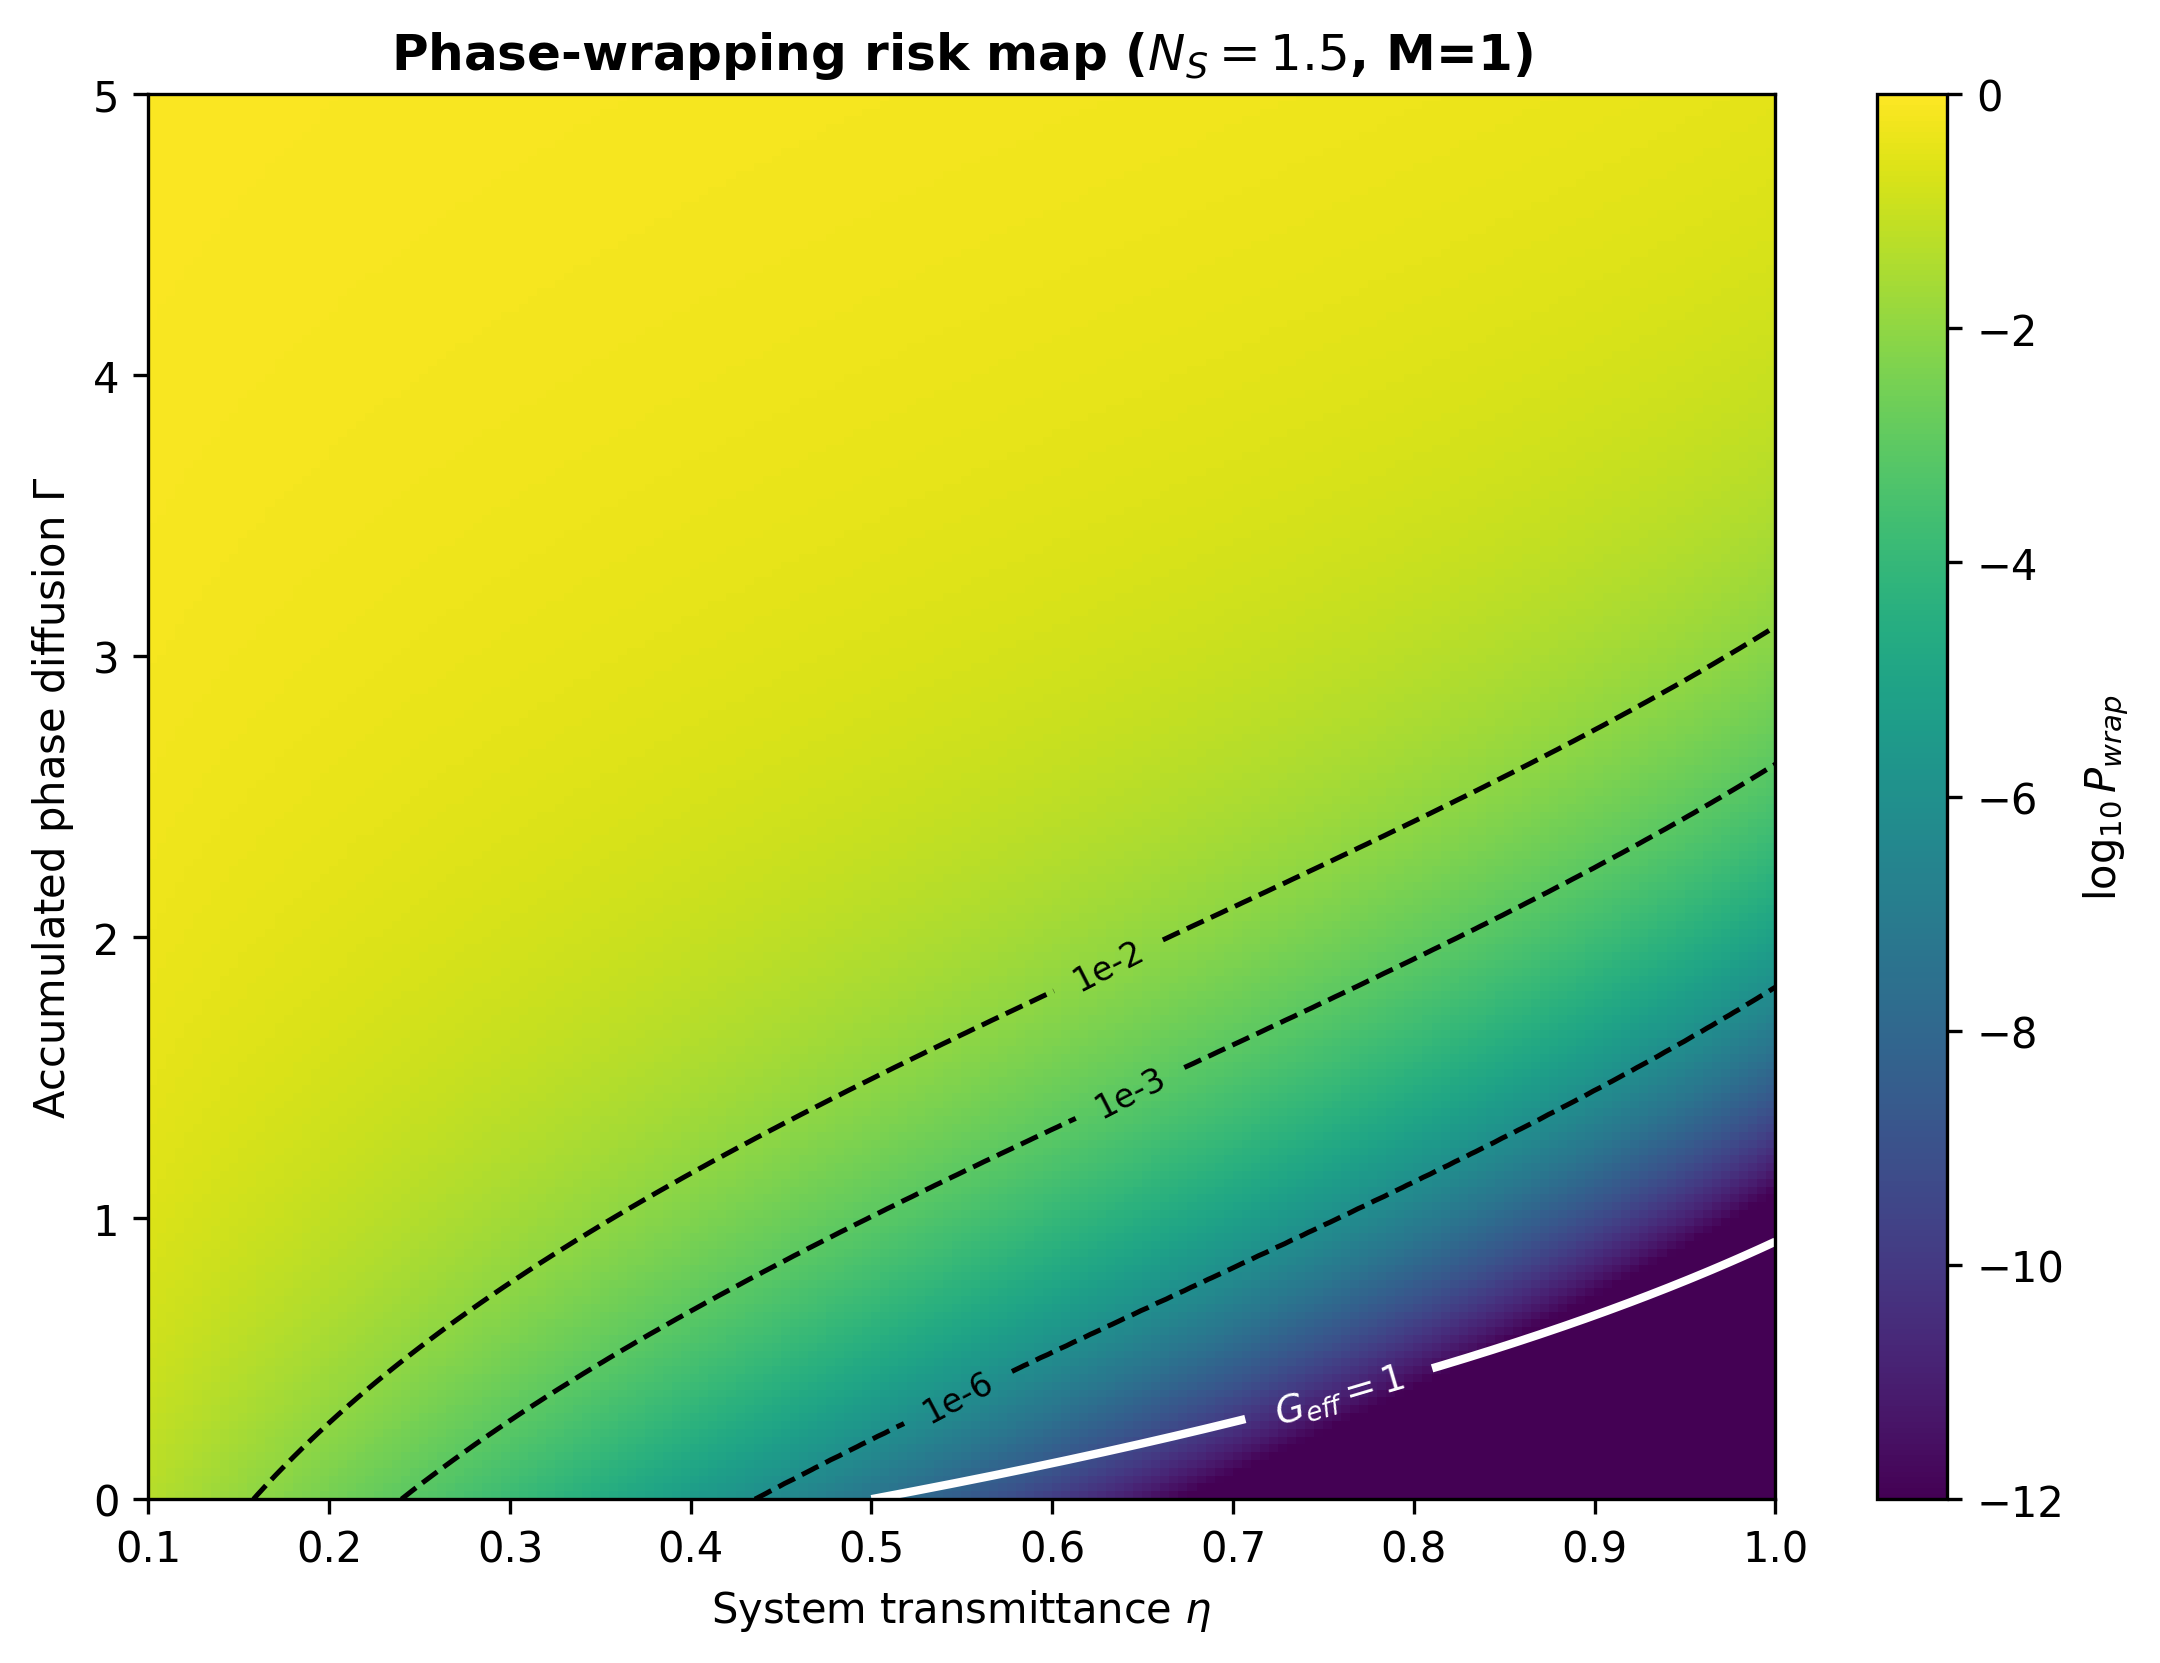
\includegraphics[width=0.82\textwidth]{phase_wrapping_risk_map.png}
  \caption{Phase-wrapping risk map under a local Gaussian phase-error approximation. $\Geff>1$ is necessary for local TMSV advantage, while sufficiently small $\Pwrap$ is separately needed for local phase interpretation.}
\end{figure}

\begin{figure}[htbp]
  \centering
  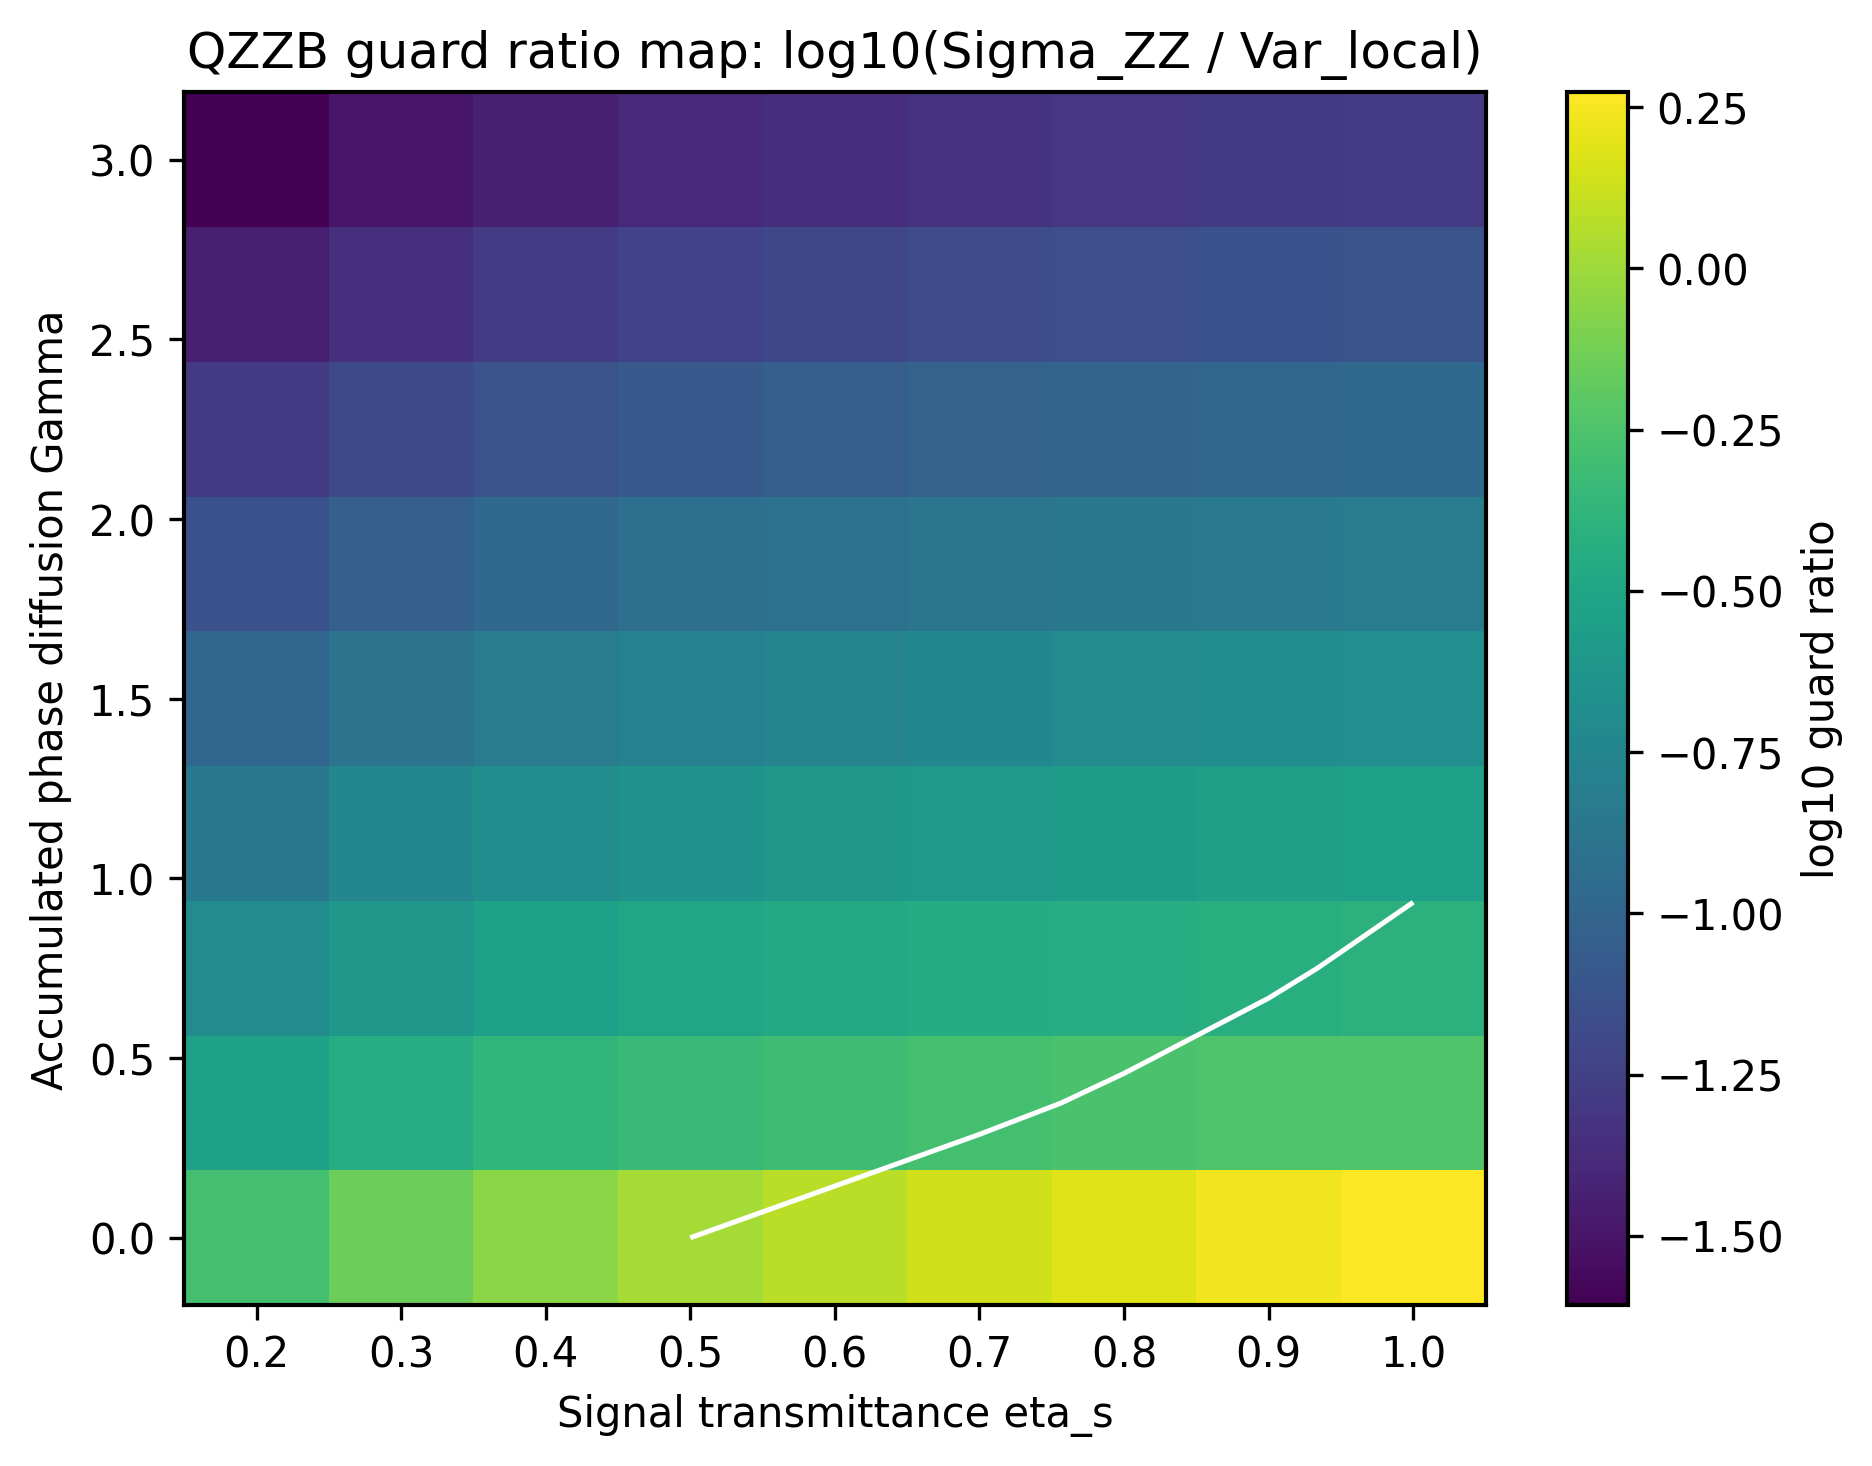
\includegraphics[width=0.75\textwidth]{figures/fig_qzzb_guard_ratio_map.png}
  \caption{QZZB guard-ratio map. The color scale shows $\log_{10}(\Sigma_{\mathrm{ZZ}}/\Var_{\mathrm{local}})$, while the white contour marks the analytic local boundary $\Geff=1$. A large guard ratio indicates that global distinguishability raises the error floor above the local QFI prediction.}
\end{figure}

\section{Detector admissibility and photon-budget anchors}
\label{app:detector_macro}

The detector scan uses Eq.~\eqref{eq:sbr} to determine whether a Rayleigh photon-budget point remains admissible at the receiver layer. This screen is deliberately separate from the TMSV QFI model. It avoids treating dark counts as an unspecified quantum-channel decoherence process and instead asks a simpler experimental question: is the returned signal above the configured detector noise floor?

\begin{figure}[htbp]
  \centering
  
\includegraphics[width=0.90\textwidth]{figures/fig_dark_count_admissibility.png}
  \caption{Detector-level dark/background-count admissibility on top of the Rayleigh photon budget. The color scale shows $\Nret/N_{\mathrm{noise}}$ for representative pressure, wavelength, and dark-count-rate settings. Crosses mark points that fail the configured detector criterion. This is a receiver-layer screen, not a modified TMSV-QFI model.}
\end{figure}

\begin{figure}[htbp]
  \centering
  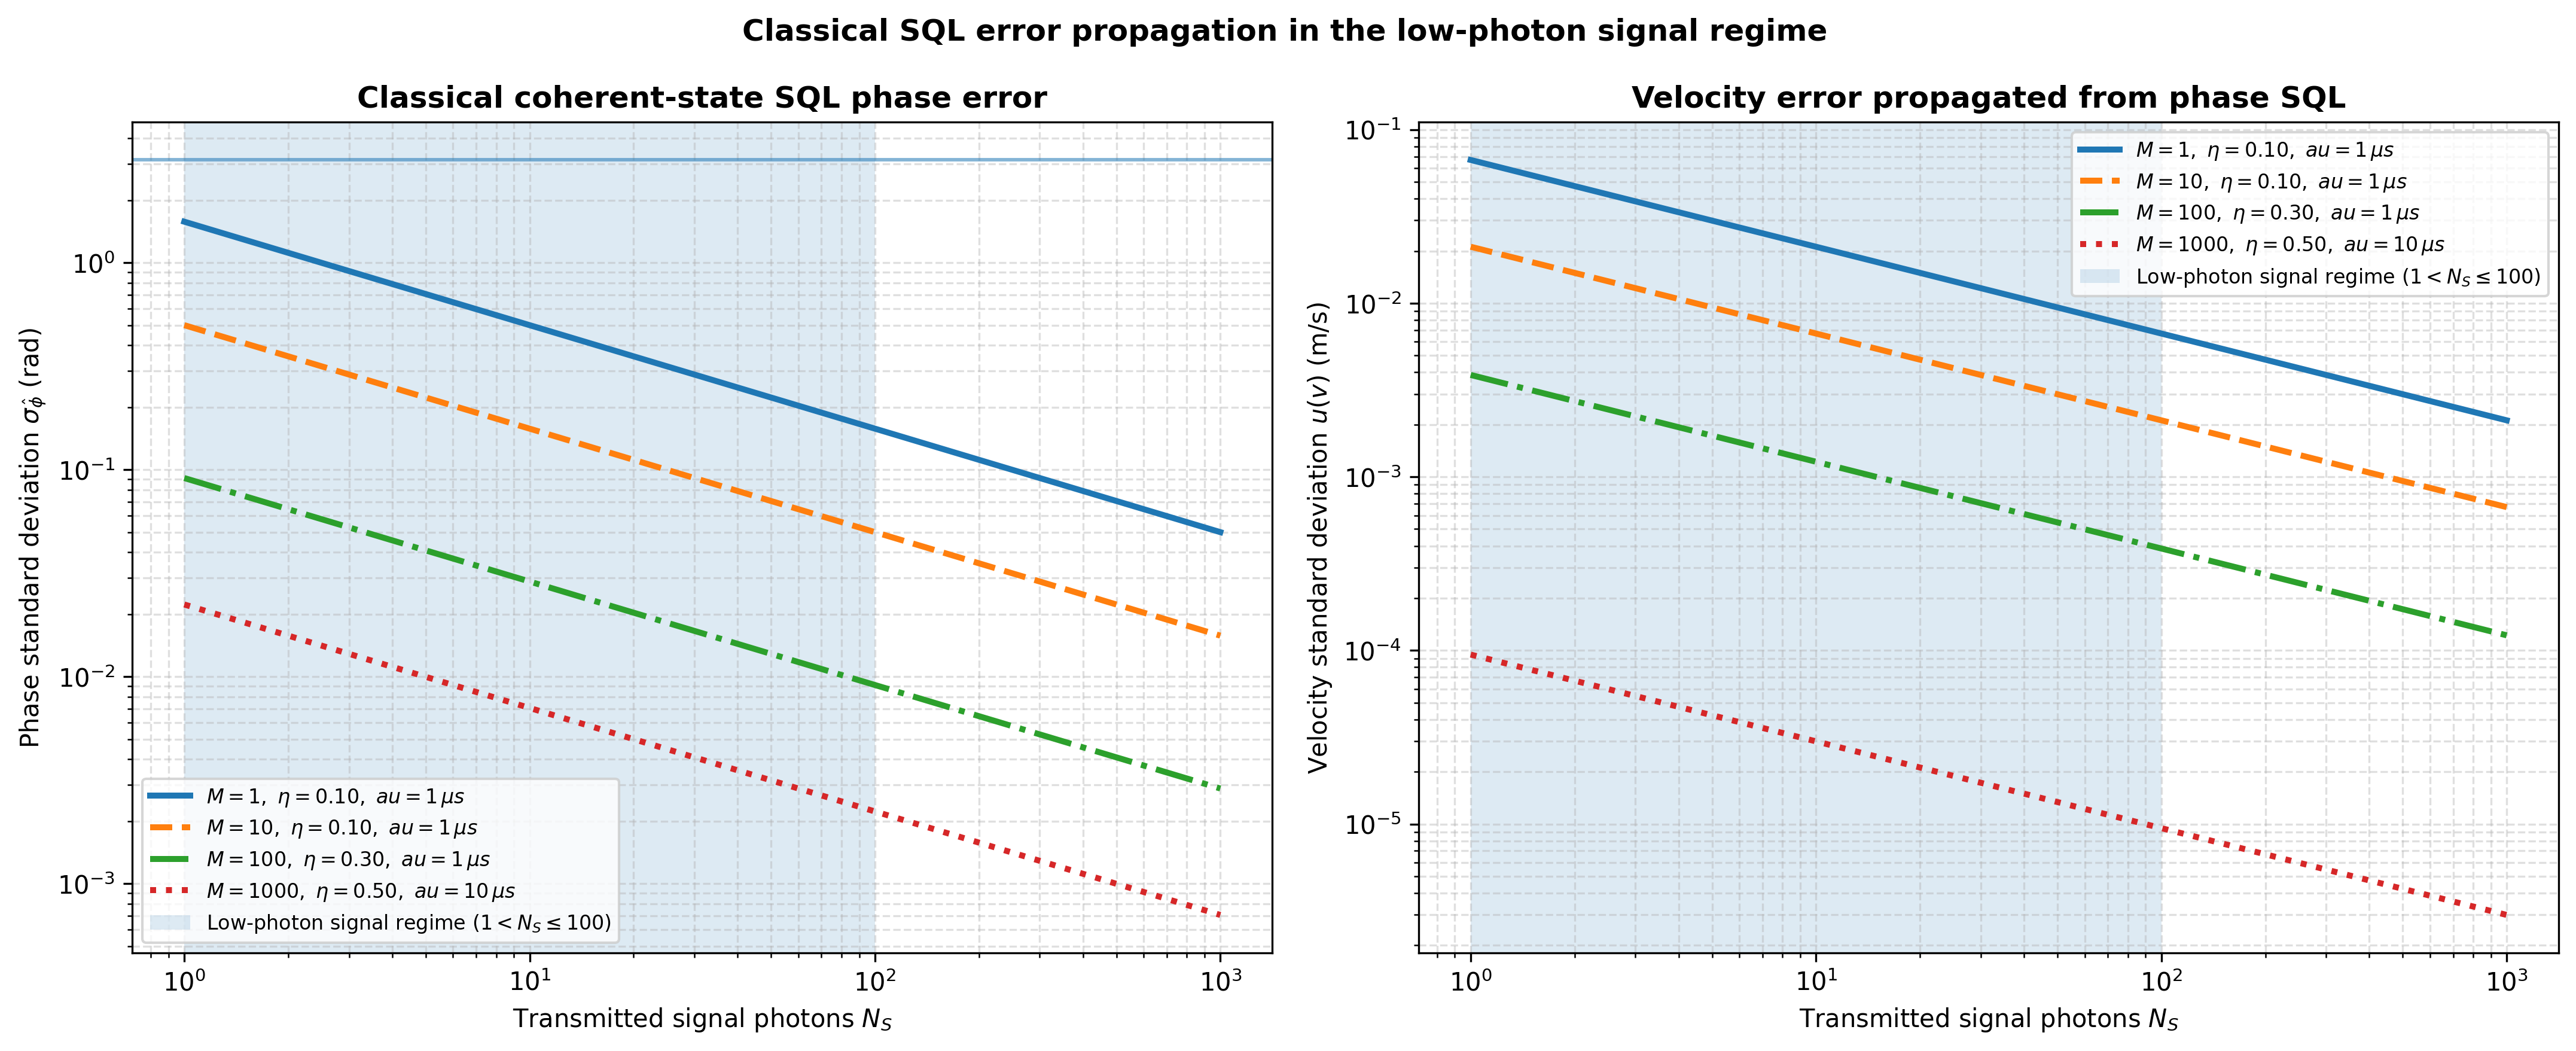
\includegraphics[width=0.75\textwidth]{fig2_classical_sql.png}
  \caption{Classical coherent-state SQL error propagation in the low-photon signal-mode regime. The shaded region refers to the microscopic signal-mode photon number $\Ns$, not the macroscopic Rayleigh return $\Nret$.}
\end{figure}

\section{Prospective uncertainty budget and macro interface}
\label{app:macro}

The microscopic phase-estimation variance enters velocity uncertainty through Eq.~\eqref{eq:phase_velocity}. If sparse quantum-assisted velocity observations are eventually used in a field-assimilation model, the reduced observation variance would enter the observation-noise covariance matrix. A schematic ensemble Kalman filter update has the form
\begin{equation}
  K_k=P_k^f H_k^T(H_kP_k^fH_k^T+R_k)^{-1},
\end{equation}
where $R_k$ contains local velocity-observation variances. This is an uncertainty-transfer interface, not an industrial EnKF validation.

\begin{table}[htbp]
\centering
\caption{Prospective GUM-style uncertainty-budget classes for future instrument-level work. It identifies classes that a future certified uncertainty budget would need to include.}
\small
\begin{tabularx}{\textwidth}{l l X}
\toprule
Source & Type & Expected propagation behavior \\
\midrule
Microscopic quantum-statistical fluctuation & A & bounded by local QCRB or guarded alternatives \\
Thermodynamic refractivity residual & B & GERG/Lorentz--Lorenz modeling uncertainty \\
Detector dark/background counts & A/B & affects receiver-layer admissibility and counting statistics \\
Window deformation and birefringence & B & alters beam angle and phase stability \\
Pressure/temperature transmitter noise & B & enters density and refractive-index inversion \\
Mode matching and idler drift & A/B & reduces retained signal--idler correlation \\
Spatial reconstruction error & A & appears if sparse local velocities are lifted to a field estimate \\
\bottomrule
\end{tabularx}
\end{table}

\begin{figure}[htbp]
  \centering
  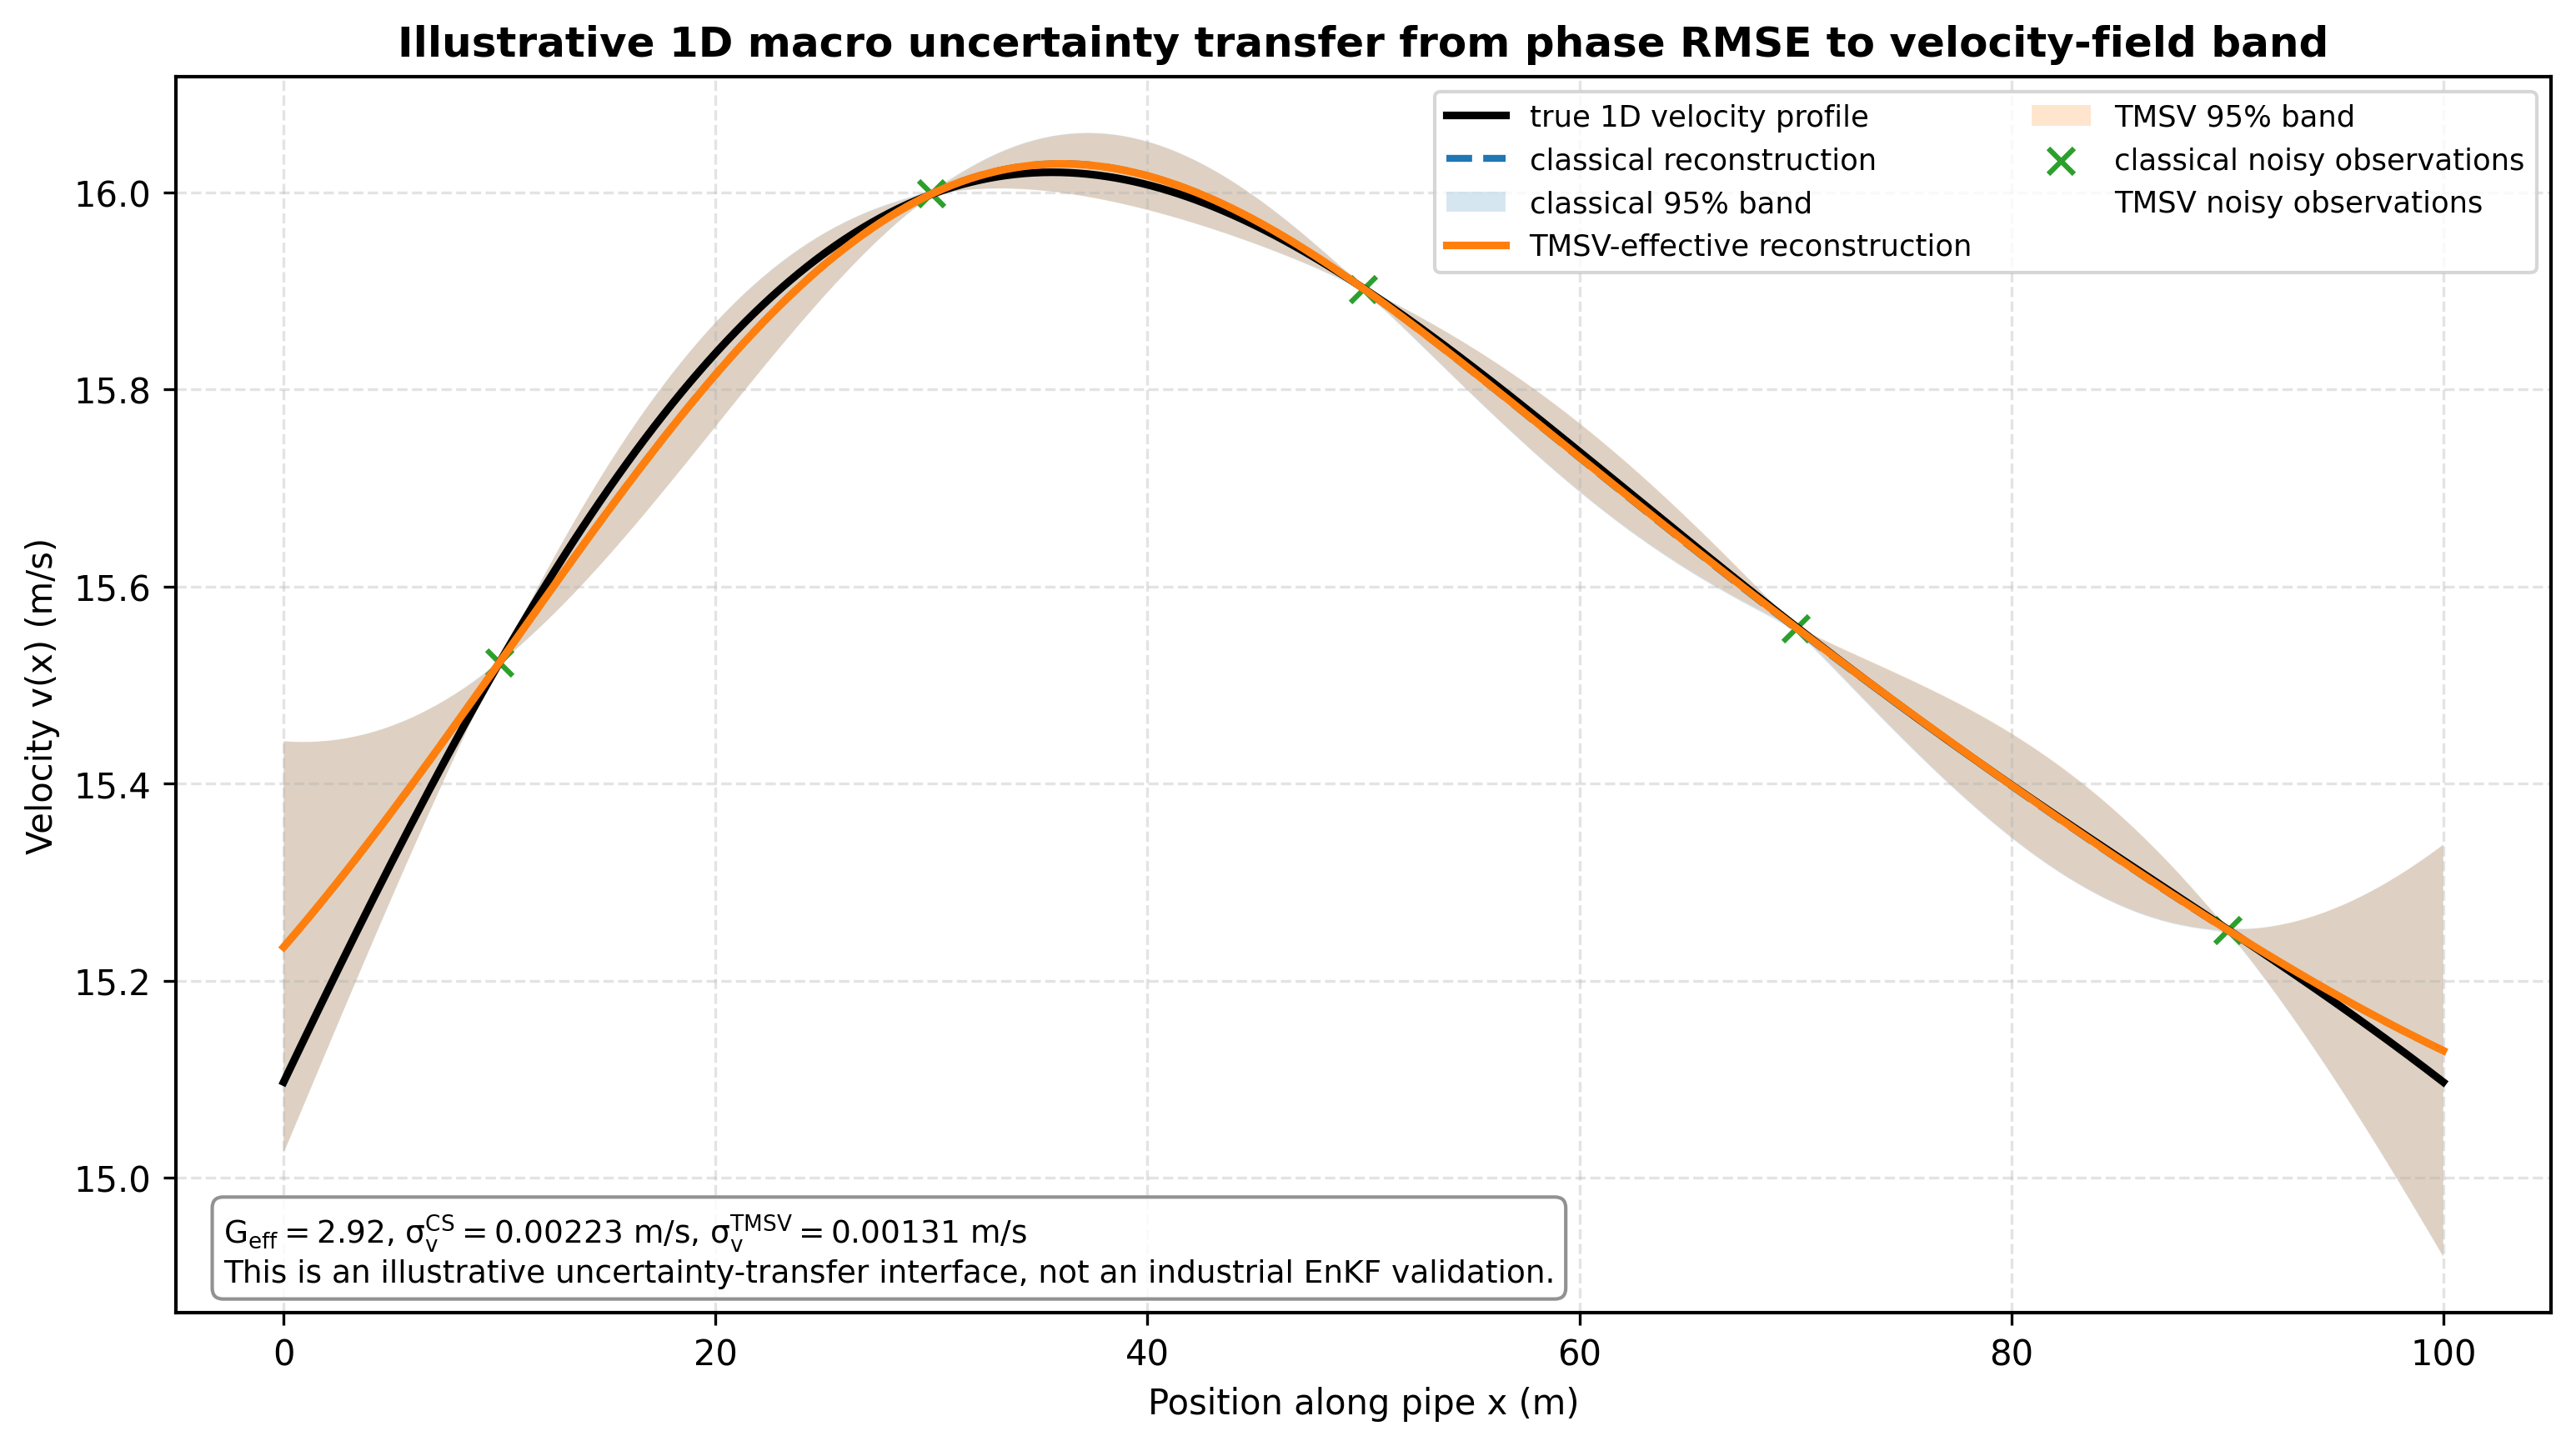
\includegraphics[width=0.84\textwidth]{figures/fig_macro_uncertainty_transfer.png}
  \caption{Illustrative 1D uncertainty-transfer example. A reduced local velocity observation noise narrows the posterior uncertainty band in a simple correlated-profile reconstruction. It is included only to show how a local variance reduction would enter a later uncertainty-transfer calculation.}
\end{figure}

\section{Reproducibility checklist}
\label{app:repro}

The numerical workflow is organized as a public Python repository rather than as manuscript source. The recommended interface is the modular \texttt{qdboundary/} package and the scripts in \texttt{scripts/}. Legacy single-file scripts may be retained for traceability, but the modular package is the final reproducibility path. The implementation uses NumPy, SciPy, and Matplotlib for arrays, numerical linear algebra, and plotting \cite{Harris2020,Virtanen2020,Hunter2007}.

\begin{verbatim}
pip install -r requirements.txt
python scripts/run_all.py --config configs/default.json
pytest
\end{verbatim}
The QZZB-certified scan is the heaviest component; the repository provides a \texttt{--skip-qzzb} option for quick checks.


\begin{table}[htbp]
\centering
\caption{Reproducibility checklist for the public code repository.}
\label{tab:repro}
\scriptsize
\renewcommand{\arraystretch}{1.15}
\begin{tabularx}{\textwidth}{p{0.22\textwidth}p{0.40\textwidth}X}
\toprule
Item & Repository file/module & Output \\
\midrule
Conceptual schematic & \texttt{scripts/00\_conceptual\_schematic.py} & system overview figure \\
Photon budget & \texttt{qdboundary/rayleigh.py}; \texttt{scripts/04\_scenario\_mapping\_table.py} & photon-regime tables \\
Pure-loss QFI & \texttt{qdboundary/formulas.py} & SQL and TMSV advantage checks \\
Phase-diffusion envelope & \texttt{scripts/01\_phase\_diffusion\_envelope.py} & $\Gamma_{\max}$ envelope and $\Geff$ map \\
Idler-loss sensitivity & \texttt{scripts/02\_idler\_loss\_sensitivity.py} & idler-loss QFI-ratio map \\
QZZB check & \texttt{qdboundary/qzzb.py}; \texttt{scripts/03\_qzzb\_certified\_phase\_diagram.py} & guard-ratio and classification maps \\
Detector admissibility & \texttt{scripts/05\_dark\_count\_admissibility.py} & dark/background-count admissibility maps \\
Multilayer map & \texttt{multilayer\_survival\_map.py} or final integrated script & multilayer admissibility map and scenario verdict table \\
Macro uncertainty interface & \texttt{scripts/06\_macro\_uncertainty\_demo.py} & illustrative 1D uncertainty-transfer figure \\
Tests & \texttt{tests/test\_core\_formulas.py} & unit-test checks \\
\bottomrule
\end{tabularx}
\end{table}



\section{Worked photon-budget anchors and multilayer failure modes}
\label{app:worked_examples}

This appendix gives the worked numerical anchors used to keep the photon-budget layer reproducible. For a selected wavelength $\lambda_0$ and pulse energy $E_p$, the emitted photons are
\begin{equation}
  N_{\mathrm{in}}=\frac{E_p}{hc/\lambda_0}.
\end{equation}
The molecular number density is obtained from the Peng--Robinson methane proxy. The Rayleigh cross section is then evaluated from Eq.~\eqref{eq:rayleigh_cross_section}, and the returned photons follow Eq.~\eqref{eq:rayleigh_budget}. The constrained optical case used throughout the manuscript has $E_p=10^{-6}\,\mathrm{J}$, $\Omega/4\pi=10^{-7}$, $\eta_{\mathrm{sys}}=0.05$, and $L=0.01\,\mathrm{m}$. At $P=30\,\mathrm{MPa}$ this gives the anchors in Table~\ref{tab:worked_anchor}. The table is not a claim of universal industrial representativeness; it is a reproducibility check for the photon-starved classification.

\begin{table}[htbp]
\centering
\caption{Constrained-case photon-budget anchors at $P=30\,\mathrm{MPa}$.}
\label{tab:worked_anchor}
\begin{tabular}{cccc}
\toprule
$\lambda_0$ (nm) & $\Nret$ & $P_0=\exp(-\Nret)$ & Regime \\
\midrule
532 & 1.2996 & 0.2726 & low-return \\
633 & 0.7715 & 0.4623 & photon-starved \\
1064 & 0.1625 & 0.8501 & photon-starved \\
1550 & 0.05255 & 0.9488 & extreme photon-starved \\
\bottomrule
\end{tabular}
\end{table}

Table~\ref{tab:expanded_verdicts} expands the scenario-level verdicts with explicit failure modes. The detector-limited case is evaluated under a harsher dark/background noise setting to make the receiver-layer veto visible. This is intentional: the table is designed to demonstrate that the multilayer framework can reject points for different reasons, not to optimize one particular instrument.

\begin{table}[htbp]
\centering
\caption{Expanded multilayer scenario verdicts. The rows are diagnostic examples showing how different layers veto or guard a nominal quantum-advantage point.}
\label{tab:expanded_verdicts}
\scriptsize
\renewcommand{\arraystretch}{1.12}
\begin{tabularx}{\textwidth}{lccccccX}
\toprule
Case & $\Nret$ & $\eta_s$ & $\eta_i$ & $\Gamma$ & $\Geff$ & Verdict & Diagnostic interpretation \\
\midrule
A green 532 & 1.30 & 0.90 & 0.90 & 0.50 & 2.92 & local-valid & low-return anchor passes detector, loss, diffusion, idler, and wrapping screens \\
B starved 1064 & 0.163 & 0.90 & 0.90 & 0.50 & 2.92 & local-valid & photon-starved but locally interpretable under the stated receiver screen \\
C noisy 1550 & 0.0526 & 0.90 & 0.90 & 0.50 & 2.92 & detector-limited & extreme photon-starved point fails under high dark/background count or large $\SBR_{\min}$ \\
D signal loss & 1.30 & 0.45 & 0.90 & 0.50 & 0.552 & stop-extrapolation & signal transmittance is below the equal-signal-energy survival threshold \\
E strong diffusion & 1.30 & 0.90 & 0.90 & 2.00 & 0.651 & stop-extrapolation & accumulated phase diffusion drives the point outside the local survival island \\
F idler poor & 1.30 & 0.90 & 0.50 & 0.50 & 2.92 & idler-limited & signal path survives, but retained idler correlation is insufficient \\
G near boundary & 1.30 & 0.75 & 0.90 & 0.70 & 1.18 & guarded & local advantage exists but the point should be treated as close to the global-check boundary \\
\bottomrule
\end{tabularx}
\end{table}

The classification algorithm used in the multilayer map is deliberately transparent. First, a fixed Rayleigh budget point is checked against detector admissibility. Second, the assumed idler efficiency is compared with an idler-preservation threshold. Third, the local boundary $\Geff>1$ is applied. Fourth, phase-wrapping risk is checked. Finally, a guard band near $\Geff=1$ is labeled guarded rather than locally interpretable. In the full QZZB-certified script, this last guard band can be replaced by the computed $\Rguard=\Sigma_{\mathrm{ZZ}}/\Var_{\mathrm{local}}$.

\section{Idler covariance diagnostics and finite-dimensional consistency}
\label{app:idler_diagnostics}

The idler-loss QFI map in Fig.~\ref{fig:idler_loss} is complemented by Gaussian covariance diagnostics. For independent signal and idler losses, the two-mode covariance matrix becomes
\begin{equation}
V(\eta_s,\eta_i)=
\begin{pmatrix}
(1+2\eta_s\Ns)I_2 & 2\sqrt{\eta_s\eta_i\Ns(\Ns+1)}Z_2\\
2\sqrt{\eta_s\eta_i\Ns(\Ns+1)}Z_2 & (1+2\eta_i\Ns)I_2
\end{pmatrix}.
\end{equation}
The Frobenius norm of the off-diagonal signal--idler block is a simple diagnostic for retained EPR-like correlation,
\begin{equation}
  \|C_{si}\|_F=\left\|2\sqrt{\eta_s\eta_i\Ns(\Ns+1)}Z_2\right\|_F.
\end{equation}
This covariance diagnostic is not a substitute for QFI, because QFI depends on how the phase parameter is encoded and on the mixed-state spectrum after loss. It is nevertheless useful for interpreting why idler loss suppresses the advantage: as $\eta_i$ decreases, the phase-sensitive correlation block shrinks even when $\eta_s$ remains moderate.

\begin{figure}[htbp]
  \centering
  
\includegraphics[width=0.74\textwidth]{figures/fig_idler_loss_covariance_correlation.png}
  \caption{Covariance-level idler-loss diagnostic. The plotted EPR block strength decreases with signal and idler loss, helping interpret why idler preservation acts as a second survival condition.}
\end{figure}

Finite-dimensional QFI calculations are sensitive to Fock cutoff when the photon-number tail is not negligible. The scripts therefore report the truncated TMSV tail probability
\begin{equation}
  P_{\mathrm{tail}}=\left(\frac{\Ns}{\Ns+1}\right)^{n_{\mathrm{cut}}},
\end{equation}
for each cutoff. For the low-dimensional diagnostic regime used in the guardrail plots, the cutoff is chosen so that the qualitative classification is stable under cutoff increase. This is weaker than a proof of high-$\Ns$ optimality, but it is the correct level of numerical check for a diagnostic guardrail.

\section{Numerical implementation notes and repository checks}
\label{app:implementation}

The final code repository is intended to be read as a reproducibility package. Its internal tests check core analytic anchors rather than every figure pixel. Representative tests include:
\begin{enumerate}[label=(\alph*)]
  \item the lossless TMSV QFI recovers $4\Ns(\Ns+1)$;
  \item the equal-signal-energy SQL boundary satisfies $\GQ(0.5,\Ns)=1$ for multiple $\Ns$ values;
  \item high loss collapses the pure-loss advantage, e.g. $\GQ(0.3,100)<1$;
  \item the Doppler conversion uses the radian wave-vector convention $K_D=4\pi n_g/\lambda_0$;
  \item scenario tables do not identify $\Nret$ with $\Ns$.
\end{enumerate}
These tests do not replace peer review of the modeling assumptions. They reduce the risk of algebraic or convention-level mistakes in the reproducibility package.

The repository also keeps legacy single-file scripts for traceability, but the recommended interface is the modular package. This distinction matters for review: the single-file scripts document the development history, while the modular package is the final reproduction path. A reviewer should be able to install the requirements, run the unit tests, and regenerate the figure/data outputs without access to the manuscript source.
\section*{Acknowledgments}

The author acknowledges the use of OpenAI's ChatGPT for language translation, text polishing, code-organization assistance, and debugging support during the preparation of this manuscript and its reproduction package. All research design, theoretical derivations, formula selection, parameter choices, numerical checks, data analysis, figures, and scientific interpretations were conducted, verified, and approved by the author, who takes full responsibility for the final content.

\begin{thebibliography}{99}
\bibitem{Durst1981} F. Durst, A. Melling, and J. H. Whitelaw, \emph{Principles and Practice of Laser-Doppler Anemometry}, 2nd ed. Academic Press, 1981.
\bibitem{Albrecht2003} H.-E. Albrecht, M. Borys, N. Damaschke, and C. Tropea, \emph{Laser Doppler and Phase Doppler Measurement Techniques}. Springer, 2003, doi:10.1007/978-3-662-05165-8.
\bibitem{Tropea2007} C. Tropea, A. L. Yarin, and J. F. Foss, eds., \emph{Springer Handbook of Experimental Fluid Mechanics}. Springer, 2007.
\bibitem{Miles2001} R. B. Miles, W. R. Lempert, and J. N. Forkey, ``Laser Rayleigh scattering,'' \emph{Measurement Science and Technology}, vol. 12, no. 5, pp. R33--R51, 2001, doi:10.1088/0957-0233/12/5/201.
\bibitem{Gu2014} Z. Gu and W. Ubachs, ``A systematic study of Rayleigh--Brillouin scattering in air, N$_2$, and O$_2$ gases,'' \emph{Journal of Chemical Physics}, vol. 141, no. 10, 104320, 2014, doi:10.1063/1.4895130.
\bibitem{Witschas2011} B. Witschas, ``Analytical model for Rayleigh--Brillouin line shapes in air,'' \emph{Applied Optics}, vol. 50, no. 3, pp. 267--270, 2011, doi:10.1364/AO.50.000267.
\bibitem{Mickan2014} B. Mickan and V. Strunck, ``A primary standard for the volume flow rate of natural gas under high pressure based on laser Doppler velocimetry,'' \emph{Metrologia}, vol. 51, no. 5, pp. 459--475, 2014, doi:10.1088/0026-1394/51/5/459.
\bibitem{Maury2018} R. Maury, A. Strzelecki, C. Auclercq, Y. Lehot, S. Loubat, J. Chevalier, F. Ben Rayana, A. A. F. Olsen, and G. Chupin, ``Cryogenic flow rate measurement with a laser Doppler velocimetry standard,'' \emph{Measurement Science and Technology}, vol. 29, no. 3, 034009, 2018, doi:10.1088/1361-6501/aa9dd1.
\bibitem{Helstrom1976} C. W. Helstrom, \emph{Quantum Detection and Estimation Theory}. Academic Press, 1976.
\bibitem{Holevo1982} A. S. Holevo, \emph{Probabilistic and Statistical Aspects of Quantum Theory}. North-Holland, 1982.
\bibitem{Giovannetti2004} V. Giovannetti, S. Lloyd, and L. Maccone, ``Quantum-enhanced measurements: beating the standard quantum limit,'' \emph{Science}, vol. 306, no. 5700, pp. 1330--1336, 2004, doi:10.1126/science.1104149.
\bibitem{Giovannetti2011} V. Giovannetti, S. Lloyd, and L. Maccone, ``Advances in quantum metrology,'' \emph{Nature Photonics}, vol. 5, pp. 222--229, 2011, doi:10.1038/nphoton.2011.35.
\bibitem{Escher2011} B. M. Escher, R. L. de Matos Filho, and L. Davidovich, ``General framework for estimating the ultimate precision limit in noisy quantum-enhanced metrology,'' \emph{Nature Physics}, vol. 7, pp. 406--411, 2011, doi:10.1038/nphys1958.
\bibitem{Demkowicz2012} R. Demkowicz-Dobrza\'nski, J. Ko\l{}ody\'nski, and M. Gu\c{t}\u{a}, ``The elusive Heisenberg limit in quantum-enhanced metrology,'' \emph{Nature Communications}, vol. 3, 1063, 2012, doi:10.1038/ncomms2067.
\bibitem{Demkowicz2015} R. Demkowicz-Dobrza\'nski, M. Jarzyna, and J. Ko\l{}ody\'nski, ``Quantum limits in optical interferometry,'' \emph{Progress in Optics}, vol. 60, pp. 345--435, 2015, doi:10.1016/bs.po.2015.02.003.
\bibitem{Pezze2018} L. Pezz\`e, A. Smerzi, M. K. Oberthaler, R. Schmied, and P. Treutlein, ``Quantum metrology with nonclassical states of atomic ensembles,'' \emph{Reviews of Modern Physics}, vol. 90, 035005, 2018, doi:10.1103/RevModPhys.90.035005.
\bibitem{BraunsteinCaves1994} S. L. Braunstein and C. M. Caves, ``Statistical distance and the geometry of quantum states,'' \emph{Physical Review Letters}, vol. 72, pp. 3439--3443, 1994, doi:10.1103/PhysRevLett.72.3439.
\bibitem{Paris2009} M. G. A. Paris, ``Quantum estimation for quantum technology,'' \emph{International Journal of Quantum Information}, vol. 7, supp. 1, pp. 125--137, 2009, doi:10.1142/S0219749909004839.
\bibitem{Monras2013} A. Monras, ``Phase space formalism for quantum estimation of Gaussian states,'' arXiv:1303.3682, 2013.
\bibitem{Safranek2019} D. \v{S}afr\'anek, ``Estimation of Gaussian quantum states,'' \emph{Journal of Physics A: Mathematical and Theoretical}, vol. 52, no. 3, 035304, 2019, doi:10.1088/1751-8121/aaf068.
\bibitem{Banchi2015} L. Banchi, S. L. Braunstein, and S. Pirandola, ``Quantum fidelity for arbitrary Gaussian states,'' \emph{Physical Review Letters}, vol. 115, 260501, 2015, doi:10.1103/PhysRevLett.115.260501.
\bibitem{Weedbrook2012} C. Weedbrook \emph{et al.}, ``Gaussian quantum information,'' \emph{Reviews of Modern Physics}, vol. 84, pp. 621--669, 2012, doi:10.1103/RevModPhys.84.621.
\bibitem{Genoni2011} M. G. Genoni, S. Olivares, and M. G. A. Paris, ``Optical phase estimation in the presence of phase diffusion,'' \emph{Physical Review Letters}, vol. 106, 153603, 2011, doi:10.1103/PhysRevLett.106.153603.
\bibitem{Altorio2015} M. Altorio, M. G. Genoni, M. D. Vidrighin, F. Somma, and M. Barbieri, ``Weak measurements and the joint estimation of phase and phase diffusion,'' \emph{Physical Review A}, vol. 92, 032114, 2015, doi:10.1103/PhysRevA.92.032114.
\bibitem{Pinel2013} O. Pinel, P. Jian, N. Treps, C. Fabre, and D. Braun, ``Quantum parameter estimation using general single-mode Gaussian states,'' \emph{Physical Review A}, vol. 88, 040102(R), 2013, doi:10.1103/PhysRevA.88.040102.
\bibitem{Tsang2012} M. Tsang, ``Ziv--Zakai error bounds for quantum parameter estimation,'' \emph{Physical Review Letters}, vol. 108, 230401, 2012, doi:10.1103/PhysRevLett.108.230401.
\bibitem{Tsang2013} M. Tsang, ``Quantum metrology with open dynamical systems,'' \emph{New Journal of Physics}, vol. 15, 073005, 2013, doi:10.1088/1367-2630/15/7/073005.
\bibitem{Lu2012} X.-M. Lu, S. Luo, and C. H. Oh, ``Hierarchy of measurement-induced Fisher information for composite states,'' \emph{Physical Review A}, vol. 86, 022342, 2012, doi:10.1103/PhysRevA.86.022342.
\bibitem{Lloyd2008} S. Lloyd, ``Enhanced sensitivity of photodetection via quantum illumination,'' \emph{Science}, vol. 321, no. 5895, pp. 1463--1465, 2008, doi:10.1126/science.1160627.
\bibitem{Tan2008} S.-H. Tan \emph{et al.}, ``Quantum illumination with Gaussian states,'' \emph{Physical Review Letters}, vol. 101, 253601, 2008, doi:10.1103/PhysRevLett.101.253601.
\bibitem{Shapiro2020} J. H. Shapiro, ``The quantum illumination story,'' \emph{IEEE Aerospace and Electronic Systems Magazine}, vol. 35, no. 4, pp. 8--20, 2020, doi:10.1109/MAES.2019.2957870.
\bibitem{Pirandola2018} S. Pirandola, B. R. Bardhan, T. Gehring, C. Weedbrook, and S. Lloyd, ``Advances in photonic quantum sensing,'' \emph{Nature Photonics}, vol. 12, pp. 724--733, 2018, doi:10.1038/s41566-018-0301-6.
\bibitem{PengRobinson1976} D.-Y. Peng and D. B. Robinson, ``A new two-constant equation of state,'' \emph{Industrial \& Engineering Chemistry Fundamentals}, vol. 15, no. 1, pp. 59--64, 1976, doi:10.1021/i160057a011.
\bibitem{KunzWagner2012} O. Kunz and W. Wagner, ``The GERG-2008 wide-range equation of state for natural gases and other mixtures: an expansion of GERG-2004,'' \emph{Journal of Chemical \& Engineering Data}, vol. 57, no. 11, pp. 3032--3091, 2012, doi:10.1021/je300655b.
\bibitem{Lorentz1880} H. A. Lorentz, ``Ueber die Beziehung zwischen der Fortpflanzungsgeschwindigkeit des Lichtes und der K\"orperdichte,'' \emph{Annalen der Physik}, vol. 245, no. 4, pp. 641--665, 1880, doi:10.1002/andp.18802450406.
\bibitem{Lorenz1880} L. Lorenz, ``Ueber die Refractionsconstante,'' \emph{Annalen der Physik}, vol. 247, no. 9, pp. 70--103, 1880, doi:10.1002/andp.18802470905.
\bibitem{JCGM2008} Joint Committee for Guides in Metrology, \emph{Evaluation of measurement data---Guide to the expression of uncertainty in measurement}, JCGM 100:2008, 2008.
\bibitem{Evensen2003} G. Evensen, ``The ensemble Kalman filter: theoretical formulation and practical implementation,'' \emph{Ocean Dynamics}, vol. 53, pp. 343--367, 2003, doi:10.1007/s10236-003-0036-9.
\bibitem{Harris2020} C. R. Harris \emph{et al.}, ``Array programming with NumPy,'' \emph{Nature}, vol. 585, pp. 357--362, 2020, doi:10.1038/s41586-020-2649-2.
\bibitem{Virtanen2020} P. Virtanen \emph{et al.}, ``SciPy 1.0: fundamental algorithms for scientific computing in Python,'' \emph{Nature Methods}, vol. 17, pp. 261--272, 2020, doi:10.1038/s41592-019-0686-2.
\bibitem{Hunter2007} J. D. Hunter, ``Matplotlib: A 2D graphics environment,'' \emph{Computing in Science and Engineering}, vol. 9, no. 3, pp. 90--95, 2007, doi:10.1109/MCSE.2007.55.
\end{thebibliography}

\end{document}
